\documentclass[article,final,14pt]{scrreprt}
\usepackage{cmap}
% \documentclass[14pt,pdf,hyperref={unicode}]{beamer}
\usepackage[utf8x]{inputenc}
\usepackage[russian]{babel}
\usepackage{amsfonts}
\usepackage{enumerate}
\usepackage{amsthm}
\usepackage{amssymb}
\usepackage{vmargin}
\usepackage{amsmath}
\usepackage{graphicx}
\usepackage{listings}
\usepackage{color}
\usepackage{multicol}
\usepackage{pb-diagram}
\usepackage[Bjornstrup]{fncychap}
\usepackage{fancyhdr}
\usepackage[svgnames,dvipsnames,x11names]{xcolor}
\usepackage{esint}
\usepackage{tocloft}
\usepackage{hyperref}
\usepackage{tikz}
\usepackage{epigraph}
\usepackage{setspace}
\usepackage{microtype}

\usetikzlibrary{calc}

\setpapersize{A4}
\setmarginsrb{2cm}{1.5cm}{1cm}{1.5cm}{0pt}{10mm}{0pt}{20mm}

\setlength\epigraphwidth{.5\textwidth}

% \usepackage[left=3.5cm,right=0cm,top=2cm,bottom=2cm]{geometry}

\usepackage{indentfirst}
\setlength{\parindent}{0.6cm}
% \sloppy

\DeclareGraphicsExtensions{.pdf,.png,.jpg}
\graphicspath{{ques/images/}}

\definecolor{linkcolor}{HTML}{610B0B}
\definecolor{urlcolor}{HTML}{6495ED}
\definecolor{lightgrey}{HTML}{9BABE7}
\definecolor{currentfancycolout}{HTML}{000000}

\hypersetup{pdfstartview=FitH,  linkcolor=linkcolor,urlcolor=urlcolor, colorlinks=true, pagecolor=linkcolor}

\setcounter{tocdepth}{2}
\linespread{1}

\fancyhead[RO]{\colorbox{currentfancycolout}{\color{white}{\textbf{\large \thepage}}}}  %% odd-right 
\fancyhead[LE]{\colorbox{currentfancycolout}{\color{white}{\textbf{\large \thepage}}}}  %%% even-left
\fancyhead[LO]{\colorbox{lightgrey}{\textbf{\thesection}}}% odd-left
\fancyhead[RE]{\colorbox{lightgrey}{\textbf{\thesection}}}% even-right 
\fancyhead[CE]{\rightmark}% odd-center, with the name of the Section
\fancyhead[CO]{\textsc{\leftmark}}% Even-center, with the name of the Chapter.
% \fancyfoot[L,R,C]{}

\makeatletter
\renewcommand*\env@matrix[1][*\c@MaxMatrixCols c]{%
  \hskip -\arraycolsep
  \let\@ifnextchar\new@ifnextchar
  \array{#1}}
\makeatother

\usepackage{enumitem}
% \setlist{noitemsep}
% \setlist[1]{\labelindent=\parindent} % < Usually a good idea
% \setlist[itemize]{leftmargin=*}
% \setlist[itemize,1]{label=$\triangleleft$}
% \setlist[enumerate]{labelsep=*, leftmargin=1.5pc}
% \setlist[enumerate,1]{label=\arabic*., ref=\arabic*}
% \setlist[enumerate,2]{label=\emph{\alph*}),
% ref=\theenumi.\emph{\alph*}}
% \setlist[enumerate,3]{label=\roman*), ref=\theenumii.\roman*}
% \setlist[description]{font=\sffamily\bfseries}

\begin{document}

\pagestyle{fancy}

% \fancyhf{} % очистили все колонтитулы
% \lhead{тратата} % левый верхний колонтитул
% \chead{} % центральный верхний
% \rhead{\textbf{\large \thepage}} % правый верхний
% \lfoot{} % левый нижний
% \cfoot{\textbf{\large \thepage}} % центральный нижний
% \rfoot{} % правый нижний

\renewcommand{\headrulewidth}{2pt} % линия под верхним к.
\renewcommand{\footrulewidth}{0pt} % линия над нижним к. 

\renewcommand\qedsymbol{$\blacksquare$}
\renewcommand\contentsname{Содержание}
\renewcommand\cftchapfont{\large\mdseries}

\newtheorem{theorem}{Теорема}[chapter]
\newtheorem{problem}{Задача}
\newtheorem{lemma}{Лемма}[chapter]
\newtheorem{clair}{Утверждение}[chapter]
\newtheorem{definition}{Определение}[chapter]
\newtheorem{propose}{Предложение}[chapter]
\newtheorem{property}{Свойство}[chapter]
\newtheorem{condition}{Условие}[chapter]
\newtheorem{properties}{Свойства}[chapter]
\newtheorem{conseq}{Следствие}[chapter]
\newtheorem{remem}{Напоминание}[chapter]
\newtheorem{example}{Пример}[chapter]
\newtheorem{rulee}{Правило}[chapter]

\newtheorem*{question}{Вопрос}
\newtheorem*{remark}{Замечание}
\newtheorem*{chck}{Проверка}
\newtheorem*{sign}{Обозначение}
\newtheorem*{uprazh}{Упражнение}

\newenvironment{Proof}       
	{\par\noindent{\bf Доказательство.}}
	{\hfill$\blacksquare$}
\newenvironment{solution}       
	{\par\noindent{\bf Решение.}}
	{\hfill$\blacksquare$}

\newcommand{\red}[1]{\textbf{\color{red}#1}}
\newcommand{\blue}[1]{\textbf{\color{blue}#1}}
\newcommand{\green}[1]{\textbf{\color{green}#1}}

\newcommand{\RNumb}[1]{\uppercase\expandafter{\romannumeral #1\relax}}

\def\ton#1{1,2,\dots,#1}
\def\Set#1#2{\left\{#1\colon#2\right\}}
\def\MYdef{\mathrel{\stackrel{\rm def}=}}
\def\QUdef{\mathrel{\stackrel{\rm ?}=}}
\def\Ddef{\mathrel{\stackrel{\rm d}=}}
\def\PNdef{\mathrel{\stackrel{\rm \text{п.н.}}=}}

\begin{titlepage}
  \begin{center}
    \large
 
  МОСКОВСКИЙ ГОСУДАРСТВЕННЫЙ УНИВЕРСИТЕТ ИМЕНИ М. В. ЛОМОНОСОВА 
    
    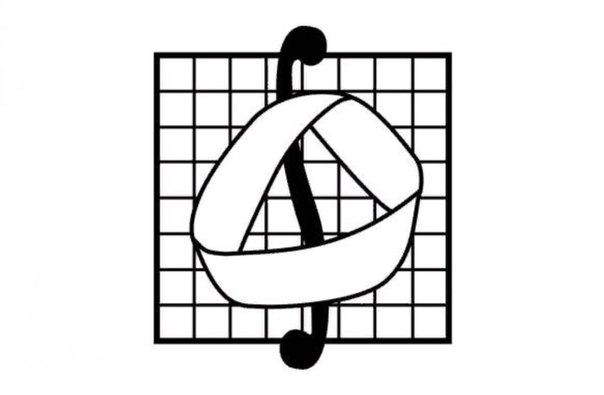
\includegraphics[scale=0.6]{mm.jpg} 
     
    Механико-математический факультет
    \vspace{0.25cm} 
      
    экономический поток
    \vspace{0.8cm} 
     
    {\LARGE МАТЕМАТИЧЕСКИЕ МЕТОДЫ В ЭКОНОМИКЕ}
    
    \vspace{0.8cm} 
    4 курс

    \vspace{0.25cm} 
    7 семестр
\end{center}
\vfill
 
\newlength{\ML}
\settowidth{\ML}{«\underline{\hspace{0.7cm}}» \underline{\hspace{1cm}}}
\hfill\begin{minipage}{7cm}
  \begin{flushright}
    Лектор $\;\;$\\
    к. ф.-м. н., доцент $\;\;$
    И.М.~Никонов $\;\;$\\
    «\underline{\hspace{0.7cm}}» \underline{\hspace{2cm}} 2021 г. $\;\;$
  \end{flushright}
\end{minipage}%
\vfill
\bigskip
 
\begin{center}
  Москва, 2021 г.
\end{center}
\tikz[remember picture,overlay] \node[opacity=0.1,inner sep=0pt] at (8.5,12.5){
\includegraphics[scale=0.8]{background1}};
\clearpage
\end{titlepage}
\newpage

\begin{center}
	{\Large \textbf{Техническая информация}}
\end{center}

\vspace{0.5cm}
Данный PDF содержит примерную программу осеннего семестра 4 курса по предмету <<Математические методы в экономике>>.

\vspace{0.5cm}
Собрали и напечатали по мотивам лекций и семинаров студенты 4-го курса Конов Марк и Гащук Елизавета.

\vspace{0.5cm}
Авторы выражают огромную благодарность лектору, кандидату ф.-м. наук, доценту Никонову Игорю Михайловичу за прочитанный курс по предмету <<Математические методы в экономике>>.

\vspace{0.5cm}
Добавления и исправления принимаются на почты \href{}{vkonov2@yandex.ru} и \\\href{}{gashchuk2011@mail.ru}.

\vspace{0.5cm}
\begin{center}
	{\Large \textbf{ПРИЯТНОГО ИЗУЧЕНИЯ}}
\end{center}

\newpage



\begin{center}
	{\Large \textbf{Программа экзамена по предмету}}
	
	{\Large \textbf{<<Алгебраические методы в экономике>>}}
\end{center}

\begin{enumerate}
	\item Описание выпуклых многогранников.
	\item Теоремы отделимости для замкнутого выпуклого множества и замкнутого
	выпуклого компакта вне него.
	\item Замкнутость конечно порожденного конуса.
	\item Теорема отделимости для замкнутого выпуклого конуса и замкнутого выпуклого компакта вне конуса.
	\item Теорема Фаркаша и ее следствия.
	\item Теорема фон Неймана.
	\item Решение игры в чистых стратегиях.
	\item Приложение теоремы фон Неймана к теории конечных антагонистических
	игр.
	\item Внутренние точки полиэдра.
	\item Грани полиэдров и экстремумы аффинных функций на полиэдрах.
	\item Грани, их размерность.
	\item Теорема Фань Цзы.
	\item Теорема Вейля. Задание многогранников системой аффинных неравенств.
	\item Симплекс-метод. Выбор главных неизвестных. Связь с вершинами полиэдра. Изменение свободных членов уравнений.
	\item Изменение системы главных неизвестных. Достаточные условия сходимости симплекс-метода.
	\item Двойственная задача линейного программирования.
	\item Совпадение ответов прямой и двойственной задач линейного программирования.
	\item Теорема о равновесии.
	\item Матричные игры как задачи линейного программирования. Решение в
	смешанных стратегиях.
	\item Критерий оптимальности допустимого плана транспортной задачи в терминах потенциалов.
	\item Построение первоначального плана. Отсутствие в нем циклов.
	\item Решение систем уравнений для потенциалов для допустимого плана в
	невырожденной задаче без циклов.
	\item Улучшение плана. Существование и единственность пути улучшения плана
	\item Отсутствие циклов в улучшенном плане.
	\item Сходимость алгоритма решения невырожденной транспортной задачи.
	\item Нормированные векторные пространства и алгебры, примеры. Индуцированные нормы на алгебре матриц.
	\item Связь нормы матрицы с ее спектральным радиусом.
	\item Оценка спектрального радиуса для неотрицательной матрицы с помощью
	элементов матрицы.
	\item Теорема о собственных векторах положительной матрицы, для которых
	собственное значение равно по модулю спектральному радиусу матрицы.
	\item Одномерность собственного подпространства положительной матрицы, со-
	ответствующего спектральному радиусу матрицы.
	\item Вычисление $\lim_m[{\rho(A)}^{−1}A]^m$ для положительной матрицы $A$.
	\item Доказать, что спектральный радиус является простым корнем характеристического многочлена положительной матрицы.
	\item Доказать, что для неотрицательной матрицы существует неотрицательный собственный вектор, собственное значение которого равно спектральному радиусу матрицы.
	\item Доказать, что неотрицательная матрица A размера n неразложима тогда
	и только тогда, когда матрица $(E + A)^{n−1}$ положительна.
	\item Теорема Фробениуса.
	\item Сходимость $[{\rho(A)}^{−1}A]^m$ для неотрицательной неразложимой матрицы.
\end{enumerate}


 

\tableofcontents

\chapter{Элементы теории потребления.}\label{cha:1}

Элементы теории потребления. Пространство товаров. Множество потребления. Отношения. Отношение предпочтения и функция полезности.

\vspace{0.5cm}

Пусть $A_1, \dots, A_n$ - различные товары в количестве $x_1, \dots, x_n$.

$\mathbb{R}_{+}^n = \Set{x \in \mathbb{R}^n}{x = (x_1, \dots, x_n), x_i \ge 0, i = \ton n}$ - положительный ортант.

\begin{definition}\label{cha:1/def:1}
	Множество $\mathbb{R}_{+}^n$, а также пространство $\mathbb{R}^n$ называются \red{пространством товаров}.
\end{definition}

\begin{clair}\label{cha:1/clair:1}
	$(x_1, \dots, x_n)$ - \red{потребительский набор} (план потребления)

	$x_i > 0$ - количество товара, которое должно быть предоставлено потребителю

	$x_j > 0$ - количество товара, предлагаемого потребителем
\end{clair}

\begin{definition}\label{cha:1/def:2}
	Множество всех планов потребления данного участника экономики называется \red{множеством потребления} $X$.
\end{definition}

\begin{remark}\label{cha:1/remark:1}
	Множество потребления $X$ учитывает физические и неэкономические ограничения.
\end{remark}

\textbf{Свойства}:
\begin{itemize}
	\item[$1$)]
		\blue{выпуклость}

		Если $x, y \in X$ и $\lambda x + (1-\lambda) y \in X \; \forall \lambda \in [0,1]$, то $X$ - выпуклое.
	\item[$2$)]
		\blue{замкнутость}

		$X$ замкнуто, если $\mathbb{R}^n \setminus X$ открыто, т.е. $\forall x \in \mathbb{R}^n \setminus X \; \exists r > 0: \; U(x, r) = \Set{y \in \mathbb{R}^n}{||x-y||_2<r} \subset (\mathbb{R}^n \setminus X)$
\end{itemize}

\begin{itemize}
	\item[$3$)]
		\blue{ограниченность}

		Пусть $x, y \in \mathbb{R}^n$, тогда:
		\begin{itemize}
			\item[$\bullet$]
				$x \le y$, если $x_i \le y_i \; \forall i = \ton n$
			\item[$\bullet$]
				$x < y$, если $x \le y$ и $x \not= y$
			\item[$\bullet$]
				$x << y$ (строго больше), если $x_i < y_i \; \forall i$
		\end{itemize}

		$X \subset \mathbb{R}^n$ ограничено сверху (снизу), если $\exists b \in\mathbb{R}^n: \; \forall x \in X \; x \le b \; (x \ge b)$.

		$X$ ограничено, если оно ограничено сверху и снизу.

		Ограниченность и замкнутость в $\mathbb{R}^n$ = компактность.

		$X$ компактно, если: $\forall \{x_k \subset X\} \; \exists$ сходящаяся подпоследовательность \\
		$x_{k_l} \underset{l \longrightarrow \infty}{\to} x: \; \forall \varepsilon > 0 \; \exists L: \; \forall l > L \; ||x - x_{k_l}|| < \varepsilon$. 
\end{itemize}

Пусть $X \subset \mathbb{R}^n$ - множество потребления. $K \in \mathbb{R}_{+}$ - капитал потребителя. $p \in \mathbb{R}_{+}^n$ - вектор цен. \\

$x = (x_1, \dots, x_n) \in X$, $p \cdot x = \underset{i=1}{\overset{n}{\sum}}p_i \cdot x_i$ - стоимость набора товаров. $p \cdot x \le K$ - бюджетные ограничения.\\

$B_{p, K} = \Set{x \in X}{p\cdot x \le K}$ - \blue{бюджетное множество} (вальрасово множество).

\begin{definition}\label{cha:1/def:3}
	Пусть $X,Y$ - множества, тогда $R \subset X \times Y$ называется (бинарным) \red{отношением}.

	$x$ находится в отношении $R$ с $y$ $(xRy)$, если $(x,y) \in R$.
\end{definition}

Отношения можно задать:
\begin{itemize}
	\item[$\bullet$] 
		матрицей $M=(m_{ij}): \; m_{ij} = \begin{cases}
			1, \; x_i R y_i \\
			0, \; (x_i, y_i) \not \in R
		\end{cases}$
	\item[$\bullet$]
		графом $x_1 \to x_2$, $(x_1, x_2) \in R$, $(x_2, x_1) \not \in R$
\end{itemize}

$\overline{D(R)} = \Set{x \in X}{\exists y \in Y: \; xRy}$ - область определения отношения $R$.

$I(R) = \Set{y \in Y}{\exists x \in X: \; xRy}$ - множество значений отношения $R$.

Если $A \subset X$, то $R(A) = \Set{y \in Y}{\exists x \in A: \; xRy}$ - образ подмножества $A$.

Если $\forall x \in X \; |R(x)| = 1$, то $R$ - однозначное отображение.\\

Пусть $X=Y$, $R \subset X\times X$ - отношение на $X$. Отношение $R$ называется:
\begin{itemize}
	\item[$1$)]
		\blue{рефлексивным}, если $\forall x \in X \; xRx$
	\item[$2$)]
		\blue{иррефлексивным}, если $\forall x \in X \; (x,x) \not \in R$
	\item[$3$)]
		\blue{симметричным}, если $\forall x, y \in X \; xRy \; \Rightarrow \; yRx$
	\item[$4$)]
		\blue{асимметричным}, если $\forall x, y \in X \; xRy \; \Rightarrow \; (y,x) \not \in R$
	\item[$5$)]
		\blue{антисимметричным}, если $\forall x, y \in X \; xRy, yRx \; \Rightarrow \; x = y$
	\item[$6$)]
		\blue{транзитивным}, если $xRy, yRz \; \Rightarrow \; xRz$
	\item[$7$)]
		\blue{полным}, если $\forall x, y, \in X \; xRy$ или $yRx$
\end{itemize}

\begin{example}\label{cha:1/example:1}
	Примеры отношений:

	Отношение эквивалентности: $1) + 3) + 6)$

	Частичный порядок: $1) + 5) + 6)$

	Линейный порядок: частный порядок $+ 7)$
\end{example}

\begin{definition}\label{cha:1/def:4}
	\red{Отношение предпочтения} - это отношение на множестве потребления, являющееся рефлексивным, транзитивным и полным ($1) + 6) + 7)$).

	Обозначение: $\preceq$
\end{definition}

\textbf{Пример} отношения $\preceq$:\\

$u: \; X \to \mathbb{R}, \; x \preceq y \; \Leftrightarrow \; u(x) \le u(y)$, $u$ - функция полезности.\\

Пусть $X$ - топологическое пространство и $\preceq$ - отношение предпочтения на $X$.

$x \prec y$, если $x \preceq y$ и $y \not \preceq x$.

$W = \Set{(x,y) \in X \times X}{x \prec y}$.

\begin{definition}\label{cha:1/def:5}
	Отношение $\prec$ называется \red{непрерывным}, если $W$ открыто в $X \times X$, т.е. $\exists$ открытые подмножества $U_{\alpha}, V_{\alpha} \subset X: \; W = \underset{\alpha}{\bigcup} U_{\alpha} \times V_{\alpha}$.

	Т.е. при малом изменении наборов $x$ и $y$ отношение сохраняется:

	$x \succ y$, $x'$ близко к $x$, $y'$ близко к $y \; \Rightarrow \; x' \succ y'$
\end{definition}

\begin{definition}\label{cha:1/def:6}
	Функция $u(x)$, определенная на множестве потребления $X$, называется \red{функцией полезности}, соответствующей отношению предпочтения $\preceq$, если $u(x) \preceq u(y) \; \Leftrightarrow \; x \preceq y$.
\end{definition}

\begin{theorem}[\red{Дебра}]\label{cha:1/the:1}
	Пусть $X \subset \mathbb{R}^n$, $\preceq$ - непрерывное отношение предпочтения, тогда $\exists$ непрерывная функция полезности $u: \; X \to \mathbb{R}$, такая, что $u$ - функция полезности для $\preceq$.
\end{theorem}

\begin{definition}\label{cha:1/def:7}
	Отношение предпочтения $\preceq$ на $X$ называют \red{локально ненасыщенным}, если $\forall x \in X$ $\exists$ открестность $U(x): \; \exists y \in U \bigcap X: \; x \prec y$, т.е. функция полезности $u(x)$ не имеет локальным максимумов на $X$.
\end{definition}

Аксиома (свойство) ненасыщенности: $x << y \; \Rightarrow \; x \prec y$.















\chapter{Задача Коши для линейного уравнения второго порядка. Теорема Коши-Ковалевской (без доказательства).}
\label{cha:2}

\begin{definition}[\red{Задача Коши}]\label{cha:2/def:1}
	\hfill \break
	Пусть $S \subset \mathbb{R}^n$ - поверхность, $dim S = n-1$, $S: F(x_1, \dots, x_n) = 0$.
	$$\begin{cases}
		\underset{i,j=1}{\overset{n}{\sum}}a_{i j} u''_{x_i x_j} + \underset{i=1}{\overset{n}{\sum}}b_i u'_{x_i} + c u = f (x_1, \dots, x_n), \;\; a_i, b_i, c, f\text{ - функции от }x_1, \dots, x_n \\
		u|_s = \varphi (\overrightarrow{x}), \; S \subset \mathbb{R}^n \\
		\frac{\partial u}{\partial \overrightarrow{l}}|_S = \psi (\overrightarrow{x}), \text{ где } \overrightarrow{l} \text{ - не касательное направление к поверхности } S
	\end{cases}$$
\end{definition}

\begin{remem}\label{cha:1/remem:1}
	\blue{Аналитическая функция} вещественного переменного - это функция, которая совпадает со своим рядом Тейлора в окрестности любой точки области определения.
\end{remem}

\begin{theorem}[\red{Коши-Ковалевской}]\label{cha:2/the:1}
	Пусть выполняется:
	\begin{itemize}
		\item[$1)$] $a_{i j} (\overline{x}), b_i (\overline{x}), c, f, \psi, \xi$ - аналитические функции в области $\Omega: s \subset \mathbb{R}$\\
		$S: F(\overline{x}) = 0 \; \Rightarrow \; F$ - тоже аналитическая функция в $\Omega$
		\item[$2)$] поверхность $S$ не характеристическая, т.е. $A(\overrightarrow{n}) \not = 0$ ни в одной точке $S$.
	\end{itemize}
	Тогда $\exists ! \; u(\overline{x})$ - решение задачи Коши в некоторой области $Q: S \subset Q \subset \Omega$ и $u(\overline{x})$ - аналитическая функция в $Q$.
\end{theorem}

\begin{remark}\label{cha:2/remark:1}
	Решение задачи Коши непрерывно зависит от начальных условий.
\end{remark}
\begin{Proof}
	Если $\varphi_n \xrightarrow[]{\text{равн-но}} \varphi, \; \psi_n \xrightarrow[]{\text{равн-но}} \psi$, то $u_n \xrightarrow[]{\text{равн-но}} u$ при $t < t_0$.\\
	$\begin{cases}
		\varphi_n(x-t) \xrightarrow[]{\text{равн-но}} \varphi (x-t) \\
		\varphi_n (x+t) \xrightarrow[]{\text{равн-но}} \varphi (x+t)
	\end{cases} \Rightarrow \; |\underset{x-t}{\overset{x+t}{\int}} \psi d\xi - \underset{x-t}{\overset{x+t}{\int}} \psi_n d\xi| \le \underset{x-t}{\overset{x+t}{\int}} |\psi - \psi_n| d\xi \le \\
	\le 2 t \cdot max |\psi - \psi_n| \to 0$, т.к. $|\psi - \psi_n| \xrightarrow[]{\text{равн-но}} 0$.
\end{Proof}


\chapter{Уравнение Слуцкого. Его следствия.}\label{cha:3}

Изучим поведение потребителя, стесненного бюджетными ограничениями.

Пусть потребительноское множество $X = \mathbb{R}_{+}^n$, функция полезности $u(x)$ гладкая и удолетворяет ограничениями:

$$\begin{gathered}
	\frac{\partial u}{\partial x_i} > 0, \; \underset{x_i \to 0}{\lim} \frac{\partial u}{\partial x_i} = \infty, \; \underset{x_i \to \infty}{\lim} \frac{\partial u}{\partial x_i} = 0, \; i = \ton n \\
	\text{Гауссиан } U(x) = \left( \frac{\partial^2 u}{\partial x_i \partial x_j} (x) \right) \text{ отрицательно определен } \forall x \in X
\end{gathered}$$

Пусть $p$ - система цен, $K$ - капитал потребителя.

Из свойств функции $u(x)$ вытекает, что функция спроса $\Phi(p, K)$ является однозначной, и при заданных $p$ и $K$ единственное значение $x^{*}(p,K)$ функции $\Phi(p,K)$ определяется следующей задачей математического программирования:
$$\begin{gathered}
	u(x) \to max \\
	< p,x > = K, \; x \ge 0
\end{gathered}$$
Кроме этого, имеем $x^{*} (p, K) >> 0$, тогда для определения точки $x^{*}(p,K)$ воспользуемся теоремой Лагранжа. Выпишем функцию Лагранжа:
$$L(x, \lambda) = u(x) - \lambda \left( <p,x> - K \right)$$
Тогда сущетсвует такое $\lambda^{*}$, что:
$$<p, x^{*}> - K = 0\eqno(1)$$
$$\frac{\partial u}{\partial x_i}(x^{*}) - \lambda^{*} p_i = 0, \; i = \ton n\eqno(2)$$

Заметим, что уравнение $(2)$ - это условие того, что бюджетная плоскость касается поверхности уровня функции полезности (градиент функции полезности сонаправлен с нормалью $p$ к бюджетной плоскости).

Рассмотрим влияение изменения цены ровно одного продукта (например, $p_n$) на поведение потребителя. Для этого продифференцируем полученные уравнения по $p_n$:
$$<p, \frac{\partial x^{*}}{\partial p_n}> = -x_n^{*}\eqno(3)$$
$$U \frac{\partial x^{*}}{\partial p_n} - \frac{\partial {\lambda}^{*}}{\partial p_n}p = (0, \dots, 0, \lambda^{*}) \MYdef \Lambda^{*}\eqno(4)$$

Воспользовавшись невырожденностью матрицы $U$ (она невырождена в силу ее отрицательной определенности), выразим из уравнения $(4)$ $\frac{\partial x^{*}}{\partial p_n}$ и подставим полученное значение в $(3)$, откуда найдем $\frac{\partial {\lambda}^{*}}{\partial p_n}$:
$$\frac{\partial {\lambda}^{*}}{\partial p_n} = -\frac{x_n^{*} + p U^{-1}\Lambda^{*}}{p U^{-1} p}$$

Обозначим $\mu = - (p U^{-1} p)^{-1}$ и $[M]^{(i)}$ - $i$-ый столбец матрицы $M$. Заметим, что $U^{-1}\Lambda^{*} = \lambda^{*} [U^{-1}]^{(n)}$. Тогда полученную формулу можно переписать так:
$$\frac{\partial {\lambda}^{*}}{\partial p_n} = \mu x_n^{*} + \mu \lambda^{*} p[U^{-1}]^{(n)}$$

Пусть $z = [U^{-1}]^{(n)}$, тогда:
$$\frac{\partial {\lambda}^{*}}{\partial p_n} = \mu x_n^{*} + \mu \lambda^{*} <z, p>$$

Отсюда получаем непосредственнуб формулу для $\frac{\partial x^{*}}{\partial p_n}$:
$$\frac{\partial x^{*}}{\partial p_n} = \mu x_n^{*} U^{-1} p + \lambda^{*} \left( \mu <p, z> U^{-1} p + z \right)\eqno(5)$$

Поймем экономический смысл правой части.

Чтобы выяснить смысл первого слагаемого, рассмотрим, что происходит с решением $x^{*}(p, K)$, если цены $p$ остаются неизменные, а капитал $K$ меняется. Продифференцируем $(1)$ и $(2)$ по $K$:
$$<p, \frac{\partial x^{*}}{\partial K}> = 1\eqno(5)$$
$$U \frac{\partial x^{*}}{\partial K} - \frac{\partial {\lambda}^{*}}{\partial K}p = 0\eqno(6)$$

Выражая из $(7)$ величину $\frac{\partial x^{*}}{\partial K}$ и подставляя полученное значение в $(6)$, найдем $\frac{\partial {\lambda}^{*}}{\partial K}$:
$$\frac{\partial {\lambda}^{*}}{\partial K} = \frac{1}{p U^{-1}p} = -\mu$$
Значит имеем:
$$\frac{\partial x^{*}}{\partial K} = -\mu U^{-1} p$$
Значит получаем:
$$\frac{\partial x^{*}}{\partial p_n} = -\frac{\partial x^{*}}{\partial K} x_n^{*} + \lambda^{*} \left( \mu <p, z> U^{-1} p + z \right)$$

Выясним теперь смысл второго слагаемого уравнения $(5)$. Для этого рассмотрим влияние компенсированного изменения цены $p$, т.е. такого изменения, при котором одновременно меняется капитал $K$ так, чтобы максимальное значение функции полезности на соответствующей бюджетной плоскости оставалось неизменным. Т.о. мы предполагаем, что капитал $K$ зависит от $p$, т.е. является функцией $K(p)$, и имеет место следующееся условие: $u(x^{*}(p, K(p))) = const$.

Рассмотрим теперь функцию $x^{*}(p,K)$ как функцию от $p$, подставив вместо $K$ соответствующую функцию $K(p)$.

\begin{definition}\label{cha:3/def:1}
	Полную производную функции $x^{*}$ по $p_j$, т.е. величину $\frac{\partial x^{*}}{\partial p_i} = \frac{\partial x^{*}}{\partial K} \cdot \frac{\partial K}{\partial p_i}$, называется \red{компенсированной производной} по $p_i$ и обозначается $\left(\frac{\partial x^{*}}{\partial p_i}\right)_{comp}$.
\end{definition}

Вычислим компенсированную производную при $i = n$. Для этого продифференцируем уравнение $(1)$ по $p_n$. Имеем:
$$x_n^{*} + \left< p, \left(\frac{\partial x^{*}}{\partial p_n}\right)_{comp} \right> - \frac{\partial K}{\partial p_n} = 0\eqno(9)$$

Т.к. при каждом $p$ функция $u(x^{*})$ остается неизменной, получаем, что вектор $\left(\frac{\partial x^{*}}{\partial p_n}\right)_{comp}$ касается поверхности $u = const$, поэтому этот вектор перпендикулярен градиенту функции $u$, т.е. вектору $\frac{\partial u}{\partial x}$. 

С другой стороны, по определению $x^{*}$, бюджетная плоскость касается в точке $x^{*}$ поверхности $u = const$, поэтому нормаль $p$ к бюджетной плоскости сонаправлена с нормальню $\frac{\partial u}{\partial x}$ к поверхности $u = const$ (из $(2)$). Значит, второе слагаемое в $(9)$ равно $0$. Отсюда получаем, что:
$$x_n^{*} = \frac{\partial K}{\partial p_n}\eqno(10)$$

Продифференцируем еще раз $(2)$ по $p_n$. Имеем:
$$U\left(\frac{\partial x^{*}}{\partial p_n}\right)_{comp} = \frac{\partial \lambda^{*}}{\partial p_n}p + \Lambda^{*}\eqno(11)$$

Воспользуемся тем, что $\left< p, \left(\frac{\partial x^{*}}{\partial p_n}\right)_{comp} \right> = 0$, выразим $\left(\frac{\partial x^{*}}{\partial p_n}\right)_{comp}$ из $(11)$ и умножим полученное выражение скалярно на $p$, найдем выражение для $\frac{\partial \lambda^{*}}{\partial p_n}$:
$$\frac{\partial \lambda^{*}}{\partial p_n} = \mu p U^{-1}\Lambda^{*} = \mu \lambda^{*} <z, p>$$

Подставим полученное выражение в $(11)$, получаем:
$$\begin{gathered}
	\left(\frac{\partial x^{*}}{\partial p_n}\right)_{comp} = \mu \lambda^{*} <z, p> U^{-1} p + U^{-1} \Lambda^{*} = \\
	= \mu \lambda^{*} <z, p> U^{-1} p + \lambda^{*} z = \lambda^{*} \left( \mu <z, p> U^{-1} p + z \right)
\end{gathered}$$

Сравнивая полученное выражение и второе слагаемое в $(5)$, получаем, что это слагаемое равно компенсированной производной функции $x^{*}$ по $p_n$. Т.о. доказали теорему.

\begin{theorem}[]\label{cha:3/the:1}
	Имеет место соотношение:
	$$\frac{\partial x^{*}}{\partial p_n} = \left(\frac{\partial x^{*}}{\partial p_n}\right)_{comp} - \left(\frac{\partial x^{*}}{\partial K}\right) x_n^{*}\eqno(12)$$
	Данное уравнение называется \red{уравнением Слуцкого}.
\end{theorem}

\textbf{Замечение}\\

Выражение для $\left(\frac{\partial x^{*}}{\partial p_n}\right)_{comp}$, полученное при выражении уравнения Слуцкого, можно пеперписать так:
$$\left(\frac{\partial x^{*}}{\partial p_n}\right)_{comp} = \lambda^{*} \left[ \mu U^{-1} p' p U^{-1} + U^{-1} \right]^{(n)}$$
где $p'$ обозначает вектор $p$, рассмтариваемый как столбец, в отличие от вектора $p$, рассматриваемого как вектор-строка.

\begin{definition}\label{cha:3/def:2}
	Матрица $H = \mu U^{-1} p' p U^{-1} + U^{-1}$ называется \red{матрицей Слуцкого}.
\end{definition}

\textbf{Свойства матрицы Слуцкого}:
\begin{itemize}
	\item[$1)$]
		\textit{матрица $H$ симметрична}
		\begin{Proof}
			$U$ - симметричная, тогда $U^{-1}$ тоже симметричная. Кроме того, матрица $p' p$ - это $n \times n$ матрица, у которой $(i, j)$-элемент равен $p_i p_j$, поэтому она тоже симметрична. Получаем:

			$$(\mu U^{-1} p' p U^{-1})^T = \mu (U^{-1})^T (p' p)^T (U^{-1})^T = \mu U^{-1} p' p U^{-1}$$

			Значит, матрица $\mu U^{-1} p' p U^{-1}$ симметрична. Т.к. сумма симметричных матриц является симметричной матрицей, то утвреждение доказано.
		\end{Proof}
	\item[$2)$]
		\textit{Имеет место соотношение: $p H = H p' = 0$}
		\begin{Proof}
			Докажем, что $p H = 0$ (второе свойство вытекает из симметричности матрицы $H$). Имеем:

			$$pH = \mu p U^{-1} p' p U^{-1} + p U^{-1} = -\frac{1}{p U^{-1}p'} (p U^{-1} p') p U^{-1} + p U^{-1} = 0$$
		\end{Proof}
	\item[$3)$]
		\textit{Матрица $H$ является полуотрицательно определенной, т.е. $\forall v \in \mathbb{R}^n \; v H v' \le 0$. Более того, $v H v' = 0 \; \Leftrightarrow$ векторы $v$ и $p$ коллинеарны.}
		\begin{Proof}
			Рассмотрим скалярное произведение с матрицей $-U^{-1}$ (она симметричная и положительно определенная), и пусть $w \in \mathbb{R}^n$ - вектор, являющийся ортогональной проекцией $v$ относительно введенного скалярного произведения на подпространство, ортогональное к $p$. Т.е. $v = \alpha p + w, \; \alpha \in \mathbb{R}$ и $w U^{-1} p' = 0$. Имеем:

			$$\begin{gathered}
				vHv' = (\alpha p + w)H(\alpha p' + w') = \alpha^2 pHp' + \alpha pHw' + \alpha wHp' + wHw' = \\
				= wHw' = w (\mu U^{-1} p' p U^{-1} + U^{-1}) w' = \\
				= \mu (w U^{-1}p')pU^{-1}w' + w U^{-1}w' = w U^{-1} w' \le 0
			\end{gathered}$$
			Равенство достигается тогда и только тогда, когда $w = 0$.
		\end{Proof}
\end{itemize}

\begin{conseq}[]\label{cha:3/conseq:1}
	Возрастание цены товара при соответствущей коменсации дохода приводит к снижению спроса на него:
	$$\left(\frac{\partial x_n^{*}}{\partial p_n}\right)_{comp} < 0$$
\end{conseq}
\begin{Proof}
	Т.к. $\left(\frac{\partial x^{*}}{\partial p_n}\right)_{comp} = \lambda^{*} [H]^{(n)}$, то $\left(\frac{\partial x_n^{*}}{\partial p_n}\right)_{comp} = \lambda^{*} h_{nn}$, где $h_{nn}$ - самый нижний диагональный элемент матрицы $H$.

	Пусть $e_i$ - базисный орт, тогда $h_{nn} = e_n H e_n$. Т.к. $p >> 0$, то $p$ и $e_n$ не коллинеарны, тогда по свойству $(3)$ матрицы Слуцкого имеем, что $h_{nn} < 0$.
\end{Proof}

\begin{definition}\label{cha:3/def:3}
	Назовем $n$-ый товар \red{ценным}, если $\frac{\partial x_n^{*}}{\partial K} > 0$, т.е. при увеличении дохода потребителя спрос на этот товар также увеличивается.

	Товар, не являющийся ценным, называется \red{малоценным}.
\end{definition}

\begin{conseq}[]\label{cha:3/conseq:2}
	Множество ценных товаров не пусто.
\end{conseq}
\begin{Proof}
	Это следует из уравнения $(6)$ и неотрицательности вектора $p$.
\end{Proof}

\begin{conseq}[]\label{cha:3/conseq:3}
	Спрос на ценные товары при повышении цены на него обязательно падает.
\end{conseq}
\begin{Proof}
	Это следует из того, что правая часть уравнения Слуцкого для $x_n^{*}$ отрицательна.
\end{Proof}

\begin{definition}\label{cha:3/def:4}
	Два товара $i$ и $j$ называются \red{взаимозаменяемыми}, если $\left(\frac{\partial x_j^{*}}{\partial p_i}\right)_{comp} > 0$, т.е. если при возрастании цены на $i$-ый товар при компенсирующем изменении дохода (с одновременным падением спроса на товар $i$) спрос на товар $j$ возрастает. 

	Если $\left(\frac{\partial x_j^{*}}{\partial p_i}\right)_{comp} < 0$, то товары $i$ и $j$ называют \red{взаимодополнительными}.
\end{definition}

\textbf{Пример}

Масло и маргарин являются взаимозаменяемыми продуктами, а бензин а автомобилями - взаимодополнительными.

\begin{conseq}[]\label{cha:3/conseq:4}
	Для каждого товара $i$ существует хотя бы один товар $j$, образующий с $i$ взаимозаменяемую пару.
\end{conseq}
\begin{Proof}
	Пусть без ограничения общности $i = n$. По следствию 3.1 имеем $\left(\frac{\partial x_n^{*}}{\partial p_n}\right)_{comp} < 0$. С другой стороны, было доказано, что $\left< \left(\frac{\partial x^{*}}{\partial p_n}\right)_{comp}, p \right> = 0$, а значит, т.к. $p >> 0$, получаем, что существует такое $j$, что $\left(\frac{\partial x_j^{*}}{\partial p_n}\right)_{comp} > 0$.
\end{Proof}

















\chapter{Правила голосования.}\label{cha:4}

Пусть $M = \{ x_1, \ldots, x_m \}$ -- множество кандидатов, $S = \{ y_1, \ldots, y_m \}$ -- множество избирателей и решение принимается голосованием. У каждого избирателя $y_k$ есть схема предпочтений: $x_{i_1} \stackrel{k}{\succ} \ldots \stackrel{k}{\succ} x_{i_m}$.

Требуется построить функцию, определяющую коллективный порядок на множестве кандидатов, то есть правило, которое для любых заданных порядков $\stackrel{1}{\succ}, \ldots \stackrel{k}{\succ}$ определяет \red{коллективный порядок} $\succeq$:

\begin{gather*}
	\succeq = f(\stackrel{1}{\succ}, \ldots \stackrel{k}{\succ}).
\end{gather*}

\begin{definition}
	$a$ -- победитель, если $\forall \; b \in M: \; a \succeq b, \; a = p (\stackrel{1}{\succ}, \ldots \stackrel{n}{\succ})$ -- правило голосования.
\end{definition}

\begin{definition}
	$\{ \stackrel{1}{\succ}, \ldots \stackrel{n}{\succ} \}$ -- профиль голосования, то есть множество всех индивидуальных предпочтений.
\end{definition}

\begin{example}
	Пусть имеется 10 избирателей и три кандидата: a, b, c. Тогда профиль голосования удобно представить таблицей:\vspace{0.5cm}

	\begin{tabular}{ | l | l | l | l | l | }
		\hline
			кол-во избирателей & 2 & 3 & 5 \\ \hline
			кандидаты & a & b & c \\
			кандидаты & b & a & b \\
			кандидаты & c & c & a \\
		\hline
	\end{tabular}
\end{example}

\begin{question}
	\textit{Как определить победителя?}
\end{question}

\begin{enumerate}
	\item \underline{Метод относительного большинства.}

	Каждый избиратель отдает голос ровно за одого кандидата, победит тот, кто наберет наибольшее число голосов.

	\item \underline{Метод абсолютного большинства.}

	Каждый избиратель голосует ровно за одного, побеждает тот, кто набрал > 50% голосов. Если такого нет или таких больше одного, проводят второй тур между кандидатами с наибольшим числом голосов.

	\item \underline{Метод Борда.}

	$y_k: \; \underset{m-1 \text{ балл}}{x_{i_1}} \stackrel{k}{\succ} \ldots \stackrel{k}{\succ} \underset{0 \text{ балл}}{x_{i_m}}$. Тогда каждому кандидату припишем балл по такой схеме: $x_{i_l} \rightarrow \alpha_{k, i_l} = m - l, $ тогда:

	\begin{gather*}
		\alpha_j = \sum \limits_{k = 1}^n \alpha_{k, i_l} \text{ -- сумма баллов для } x_j.
	\end{gather*}

	Тогда победитель - это тот, кто имеет наибольшее $\alpha_j.$

	\item \underline{Обобщенный метод Борда.}

	$y_k: \; x_{i_1} \stackrel{k}{\succ} \ldots \stackrel{k}{\succ} x_{i_m}, \; x_{i_l} \rightarrow \alpha_{k, i_l} = s_{m - l}: \; 0 = s_0 \leq s_1 \leq \ldots \leq s_{m - 1} > 0,$ дальше аналогично методу Барда из пункта 3.

	\begin{remark}
		\begin{itemize}
			\item $s_{m - l} = m - l$ -- обычный метод Борда.
			\item $s_0 = \ldots = s_{m - 2} = 0, \; s_{m - 1} = 1$ -- метод относительного большинства.
		\end{itemize}
	\end{remark}

	\item \underline{Метод Кондорсе.}

	$a, \; b \in M $ -- кандидаты. $K_{a, b}$ -- количество избирателей, считающих a лучше b: 

	\begin{gather*}
		r_a := \{ \#(b \in M\setminus\{ a \}) \mid K_{a, b} \geq K_{b, a} \},
	\end{gather*}

	где $\#$ -- количество. Тогда победитель -- кандидат с наибольшим $r_a$.
\end{enumerate}

\begin{example}

	\begin{tabular}{ | l | l | l | l | }
		\hline
			5 & 3 & 5 & 4 \\ \hline
			a & a & b & c \\
			d & d & c & d \\
			c & b & d & b \\
			b & c & a & a \\
		\hline
	\end{tabular}\vspace{0.5cm}
	\begin{enumerate}
		\item $a \rightarrow 8, \; b \rightarrow 5, \; c \rightarrow 4, \; d \rightarrow 0 \Rightarrow $ победитель -- а.
		\item $8 < \dfrac{17}{2} \Rightarrow $ проводим второй тур между $a, \; b:$

		\begin{table}[h!]
		\caption{Второй тур}
		\begin{center}
		\begin{tabular}{ | l | l | l | l | }
			\hline
				5 & 3 & 5 & 4 \\ \hline
				a & a & b & b \\
				b & b & a & a \\
			\hline
		\end{tabular}
		\end{center}
		\end{table}\vspace{0.5cm}

		Тогда победитель -- b.\vspace{0.5cm}

		\item 

		\begin{tabular}{ | l | l | l | l | l | }
		\hline
			5 & 3 & 5 & 4 & баллы\\ \hline
			a & a & b & c & 3 \\
			d & d & c & d & 2 \\
			c & b & d & b & 1 \\
			b & c & a & a & 0 \\
		\hline
		\end{tabular}\vspace{0.5cm}

		$\alpha_a = 5 \cdot 3 + 3 \cdot 3 + 5 \cdot 0 + 4 \cdot 0 = 24$

		$\alpha_b = 5 \cdot 0 + 3 \cdot 1 + 5 \cdot 3 + 4 \cdot 1 = 22$

		$\alpha_c = 5 \cdot 1 + 3 \cdot 0 + 5 \cdot 2 + 4 \cdot 3 = 27$

		$\alpha_d = 5 \cdot 2 + 3 \cdot 2 + 5 \cdot 1 + 4 \cdot 2 = 29$\vspace{0.5cm}

		Тогда победитель -- d.

		\item -

		\item $a \preceq b: \; 8:9$

		$a \preceq c: \; 8:9$

		$b \preceq c: \; 8:9$

		$d \preceq c: \; 8:9$

		$a \preceq d: \; 8:9$

		$b \preceq d: \; 5:12$\vspace{0.5cm}

		Поэтому $r_a = 0, \; r_b = 1, \; r_c = 3, \; r_d = 2 \Rightarrow $ победитель -- c.

	\end{enumerate}	

	\begin{clair}
		Методы 1), 2), 3), 5) различны.
	\end{clair}
\end{example}\newpage

\begin{example}

	\begin{tabular}{ | l | l | l | l | }
		\hline
			3 & 6 & 4 & 4\\ \hline
			c & a & b & b\\
			a & b & a & c\\
			b & c & c & a\\
		\hline
	\end{tabular}\vspace{0.5cm}

	5). $b \preceq a: \; 8:9$

	$c \preceq a: \; 7:10$\vspace{0.5cm}

	Победитель -- a.\vspace{0.5cm}

	4). $\alpha_a = 6s_2 + 7s_1$

	$\alpha_b = 8s_2 + 6s_1$

	$\alpha_a = 3s_2 + 4s_1$\vspace{0.5cm}

	Пусть побеждает a $ \Rightarrow 6s_2 + 7s_1 \geq 8s_2 + 6s_1 \Rightarrow s_1 \geq 2s_2$ и $ 6s_2 + 7s_1 \geq 3s_2 + 4s_1 \Rightarrow s_2 \geq s_1.$ Тогда

	\begin{gather*}
		s_1 \geq 2s_2 \geq 2s_1 \Rightarrow s_1 = s_2 \text{ -- противоречие.}
	\end{gather*}

	\begin{clair}
		Методы 2), 5) не являются частными случаями обобщенного метода Борда.
	\end{clair}

\end{example}
\chapter{Функции коллективного выбора. Теорема Эрроу.}\label{cha:5}

Пусть $S = \{y_1, \dots, y_n\}$ - множество избирателей, $M = \{x_1, \dots, x_m\}$ - множество кандидатов. Т.о. имеем $n$ систем индивидуального предпочтения, каждая из которых устанавливает линейный порядок на множестве всех кандидатов.

Пусть $p$ - произвольное правило голосования. Применяя правило $p$, построим множество $M_1 = \{a_1 = \dots = a_s\}$, состоящее из победителей. 

Применим правило $p$ ко множеству проигравших $M \setminus M_1$. Опять получаем множество выигравших $M_2 = \{a_{s+1} = \dots = a_{s+l}\}$.

Выкинем из $M$ объединение $M_1 \bigcup M_2$ и проделаем ту же операцию, и т.д. В результате мы упорядочим множество $M$ согласно решению коллектива: 
$$M_1 \succ M_2 \succ \dots$$

Таким образом, правило голосования позволяет построить систему коллективного предпочтения. И из правила $p$ строим \red{функцию коллективного предпочтения} $\succeq = f(\overset{1}{\succ}, \dots, \overset{n}{\succ})$, где $\overset{k}{\succ}$ - система индивидуального предпочтения.

\textbf{Требования} к функции коллективного предпочтения:
\begin{itemize}
	\item[$1$.]
		\blue{полнота}

		Для любых кандидатов $a$ и $b$ коллективный порядок устанавливает, что либо $a \prec b$, либо $b \prec a$, либо $a = b$.
	\item[$2$.]
		\blue{транзитивность}

		Для любых трех кандидатов $a, b, c$ таких, что $a \preceq b$ и $b \preceq c$, выполняется $a \preceq c$, причем равенство имеет место, если и только $a = b = c$.
	\item[$3$.]
		\blue{единогласие}

		Если все избиратели считают, что $a$ лучше $b$, значит и в коллективном предпочтении $a$ должен быть лучше $b$:
		$$\forall k \; a \overset{k}{\prec} b \; \Rightarrow \; a \prec b$$
	\item[$4$.]
		\blue{независимость}

		Положение любых двух кандидатов в коллективном предпочтении зависит только от их взаимного расположения в индивидуальных предпочтениях и не зависит от расположения других кандидатов. 

		Т.о. если для профиля вида:
		\begin{tabular}{ | c | c | }
			\hline
				группы избирателей & кандидаты \\ \hline
				$A$ & $\cdot \cdot \cdot$ $a$ $\cdot \cdot \cdot$ $b$ $\cdot \cdot \cdot$ \\
				$S \setminus A$ & $\cdot \cdot \cdot$ $b$ $\cdot \cdot \cdot$ $a$ $\cdot \cdot \cdot$ \\
			\hline
		\end{tabular}
		имеем $a \prec b$, то и для всех профилей такого вида $a \prec b$.
\end{itemize}

\begin{remark}\label{cha:5/remark:1}
	Множество функций коллективного выбора, удовлетворяющих аксимомам 1-4, непусто. Примером таких функций могут служить \red{функции диктатора}, а именно функции вида $f(\overset{1}{\succ}, \dots, \overset{n}{\succ}) = \overset{k}{\succ}$ для некоторого $k$. 
\end{remark}

\begin{theorem}[\red{Эрроу}]\label{cha:5/the:1}
	Пусть $f$ - функция коллективного предпочтения, удовлетворяющая аксиомам 1-4, и предположим, что имеется не менее 3 кандидатов. Тогда $f$ - функция диктатора.

	(диктатура описывается аксиомами, а демократия - отрицание диктатуры)
\end{theorem}
\begin{Proof}
	Введем некоторые понятия.

	Произвольное подмножество $A$ множества избирателей называется \blue{коалицией}.

	\begin{definition}\label{cha:5/def:1}
		Коалиция $A$ назывется \blue{f-решающей для кандидата $a$ против кандидата $b$}, тогда и только тогда, когда из того, что все члены коалиции $A$ ставят $a$ выше $b$, а все члены, не входящие в $A$, ставят $b$ выше $a$, вытекает, что в коллективном предпочтении $a \prec b$:
		$$(\forall y_k \in A, \; a \overset{k}{\prec} b) \bigcup (\forall y_k \not \in A, \; b \overset{k}{\prec}a) = a \prec b$$
		Обозначение: $A = f(a, b)$.
	\end{definition}

	Коалиция $A$, такая, что для любых двух кандидатов $a$ и $b$ коалиция $A$ является $f$-решающей для $a$ против $b$ назывется просто \blue{$f$-решающей}.

	\begin{lemma}[]\label{cha:5/lemma:1}
		$\exists$ пара кандидатов $(a, b)$, для которой найдется коалиция $D$, состоящая из одного избирателя $d$, такая, что $D = f(a, b)$.
	\end{lemma}
	\begin{Proof}
		Обозначим через $K$ множество всех коалиций, для каждой из которых $\exists$ пара кандидатов $(a, b)$, таких, что эта коалиция является $f$-решающей для $a$ против $b$. 

		Отметим, что множество $K$ не пусто, т.к., в силу аксиомы единогласия, множество всех избирателей $S$ образует $f$-решающую коалицию $\forall$ пары кандидатов $(a, b)$.

		Рассмотрим в $K$ коалицию $D$, состоящую из наименьшего числа избрателей. Покажем, что $D$ состоит ровно из одного элемента.

		Предположим противное, т.е. $D = \{d\} \bigcup E$, где $E$ - некоторое непустое множество кандидатов. Если $S$ состоит из $\ge 2$ кандидатов, рассмотрим профиль:

		\begin{center}
			\begin{tabular}{ | c | c | c | c |}
				\hline
					группа избирателей & $\{d\}$ & $E$ & $S \setminus D$ \\ \hline
					кандидаты & $a$ & $c$ & $b$ \\
					кандидаты & $b$ & $a$ & $c$ \\
					кандидаты & $c$ & $b$ & $a$ \\
				\hline
			\end{tabular}
		\end{center}

		Если же $S$ состоит из двух кандидатов, рассмотрим профиль:

		\begin{center}
			\begin{tabular}{ | c | c | c |}
				\hline
					группа избирателей & $\{d\}$ & $E$ \\ \hline
					кандидаты & $a$ & $c$ \\
					кандидаты & $b$ & $a$ \\
					кандидаты & $c$ & $b$ \\
				\hline
			\end{tabular}
		\end{center}

		Т.к. $D = f(a,b)$, то $a \prec b$. Предположим, что $c \prec b$. Тогда $E = f(c, b)$, что противоречит минимальности коалиции $D$. Значит, $b \preceq c$, и, по аксиоме транзитивности, $a \prec c$. Но тогда $\{d\} = f(a,c)$, что опять же противоречит минимальности коалиции $D$.

		Т.о., мы получили противоречие к предположению, что $D$ состоит из $\ge 1$ элемента, а значит, $D$ содержит ровно $1$ элемент.
	\end{Proof}

	\begin{lemma}[]\label{cha:5/lemma:2}
		Коалиция $D$ из леммы $5.1$ является $f$-решающей.
	\end{lemma}
	\begin{Proof}
		Пусть $c$ - произвольный кандидат. Рассмотрим профиль:

		\begin{center}
			\begin{tabular}{ | c | c | }
				\hline
					группы избирателей & кандидаты \\ \hline
					$\{d\}$ & $\dots a \prec \dots \prec b \prec \dots \prec c \dots$ \\
					$S \setminus \{d\}$ & $\dots b \prec \dots \prec c \prec \dots \prec a \dots$ \\
				\hline
			\end{tabular}
		\end{center}

		Т.к. $\{d\} = f(a,b)$, то $a \prec b$. В силу аксиомы единогласия, $b \prec c$, значит, по транзитивности, $a \prec c$. Значит, $\{d\} = f(a, c)$.

		Пусть $e$ - еще один кандидат. Рассмотрим профиль:

		\begin{center}
			\begin{tabular}{ | c | c | }
				\hline
					группы избирателей & кандидаты \\ \hline
					$\{d\}$ & $\dots e \prec \dots \prec a \prec \dots \prec c \dots$ \\
					$S \setminus \{d\}$ & $\dots c \prec \dots \prec e \prec \dots \prec a \dots$ \\
				\hline
			\end{tabular}
		\end{center}

		По аксиоме единогласия, $e \prec a$. Т.к. $a \prec c$, то по транзитивности для данного профиля имеем $e \prec c$. Но тогда $\{d\} = f(e,c)$.

		Т.о. мы показали, что для любых двух кандидатов $e$ и $c$ коалиция $\{d\}$ является $f$-решающей для $e$ против $d$. Значит, коалиция $\{d\}$ есть $f$-решающая коалиция.
	\end{Proof}

	\begin{lemma}[]\label{cha:5/lemma:3}
		Избиратель $d$ является диктатором.
	\end{lemma}
	\begin{Proof}
		Мы показали, что $d$ может навязывать свое мнение по поводу любых двух кандидатов $a$ и $b$ при условии, что мнение остальных избирателей противоположно - в этом пока проявляется зависимость от мнения других.

		Надо показать, что как бы не голосовали остальные избиратели, коллективное мнение совпадает с мнением $d$. \\

		Рассмотрим такие профили голосования, в которых у избирателя $d$ порядок вида $\dots a \overset{d}{\prec} \dots \overset{d}{\prec} c \overset{d}{\prec} \dots \overset{d}{\prec} b \dots$, а все остальные избиратели ставят $c$ выше, чем $a$ и $b$.

		Т.к. $\{d\}$ является $f$-решающей коалицией, то для таких профилей $a \prec c$. В силу аксиомы единогласия $c \prec b$, тогда по транзитивности $a \prec b$. 

		Исключая из соотношений $c$ и используя аксиому независимости, получаем, что если $d$ ставит $a$ выше $b$, то и в коллективном порядке $a \prec b$. В силу произвольности $a$ и $b$, получаем, что $d$ - диктатор.
	\end{Proof}

	Доказательство теоремы закончено.
\end{Proof}


















\chapter{Теорема фон Неймана}
\label{cha:6}

\epigraph{
	\textit{И опять в неясную и мутную молитву отчетливо, выпукло, звонко врывалась кощунственная фраза…}}
{-- Короленко В.Г.}

\begin{propose}\label{cha:6/propose:1}
	Пусть множество точек $T \subseteq \mathbb{A}^n$ – компактно и выпукло, $N'$ – компактное выпуклое множество аффинных функций на $\mathbb{A}^n$. Предположим, что для любой точки $a \in T$ найдется такая функция $f \in N'$, что $f(a) \ge 0$. Тогда существует такая аффинная функция $f_0 \in N'$, что $f_0 |_T \ge 0$.
\end{propose}
\begin{Proof}
	Обозначим через K – множество всех аффинных функций на $\mathbb{A}^n$, принимающих на T неотрицательные значения. Тогда K является замкнутым выпуклым конусом в линейном пространстве всех аффинных функций.

	\begin{lemma}\label{cha:6/lemma:1}
		Пусть $b \in \mathbb{A}^n$ и $f(b) \ge 0$ для всех $f \in K$. Тогда $b \in T$.
	\end{lemma}
	\begin{Proof}
		Если бы $b \not \in T$, то по теореме \ref{cha:5/the:1} существовала бы такая аффинная функция f, что $f |_T \ge 0$ и $f(b) < 0$. Эта функция f принадлежит K. Получается противоречие с условием леммы.
	\end{Proof}

	Продолжим доказательство предложения. Предположим, что $K \cap N' = \emptyset$. Выберем в $\mathbb{A}^n$ систему координат $O, e_1, \dots, e_n$. Каждая аффинная функция f представляется в виде $f(x) = a_0 + \underset{i}{\overset{}{\sum}} a_i x_i$. По предложению \ref{cha:6/propose:1} существует такая аффинная функция $h(z) = \underset{i=0}{\overset{n}{\sum}} b_i z_i$ на пространстве аффинных функций на $\mathbb{A}^n$, что $h(f) = \underset{i=0}{\overset{n}{\sum}} b_i a_i \ge 0$ для всех $f \in K$ и $h(g) < 0$ для всех $g \in N'$. Так как функция $f = 1$ лежит в K, то $h(1) = b_0 \ge 0$.

	Предположим, что $b_0 > 0$. Тогда точка $b = \left( \frac{b_1}{b_0}, \dots, \frac{b_n}{b_0} \right)$ обладает тем свойством, что $f(b) = \frac{1}{b_0} h(f) \ge 0$ для всех $f \in K$ и поэтому в силу леммы \ref{cha:6/lemma:1} получаем $b \in T$. С другой стороны, $g(b) = b_0^{−1} h(g) < 0$ для всех $g \in N'$, что противоречит условиям предложения.

	Предположим теперь, что $b_0 = 0$. В этом случае:
	$$\begin{gathered}
		h(f) = \underset{i=1}{\overset{n}{\sum}}b_i a_i \ge 0, \; h(g) = \underset{i=1}{\overset{n}{\sum}}b_i c_i < 0 \\
		\text{для всех } f = a_0 + \underset{i=1}{\overset{n}{\sum}}a_i x_i \in K, \; g = c_0 + \underset{i=1}{\overset{n}{\sum}}c_i x_i \in N'
	\end{gathered}$$
	В частности, $b \not = 0$. Возьмем точку $z = (z_1, \dots, z_n) \in T$. Для любого $\mu \ge 0$ и любого $f \in K$ получаем:
	$$f(z + \mu b) = a_0 + \underset{i=1}{\overset{n}{\sum}}a_i z_i + \mu \underset{i=1}{\overset{n}{\sum}}a_i b_i \ge 0$$
	По лемме \ref{cha:6/lemma:1} точка $z + \mu b \in T$ для всех $\mu \ge 0$. Но это противоречит компактности T, поскольку $b \not = 0$. Следовательно, $K \cap N'$ непусто.
\end{Proof}

\begin{propose}\label{cha:6/propose:2}
	Пусть заданы компактные замкнутые выпуклые подмножества $N \subseteq \mathbb{A}^n$, $M \subseteq \mathbb{A}^m$ и $F (x, y)$ – непрерывная функция, где $x \in N$, $y \in M$. Тогда:
	$$\underset{x \in N}{\max} \; \underset{y \in M}{\min} F(x,y) \le \underset{y \in M}{\min} \; \underset{x \in N}{\max} F(x, y)$$
\end{propose}
\begin{Proof}
	$$\begin{gathered}
		F(x,y) \le \underset{x \in N}{\max} F(x,y) \; \Rightarrow \; \underset{y \in M}{\min} F(x,y) \le \underset{y \in M}{\min} \; \underset{x \in N}{\max} F(x,y) \; \Rightarrow \\
		\Rightarrow \; \underset{x \in N}{\max} \; \underset{y \in M}{\min} F(x,y) \le \underset{y \in M}{\min} \; \underset{x \in N}{\max} F(x, y)
	\end{gathered}$$
\end{Proof}

\begin{theorem}[\red{фон Неймана}]\label{cha:6/the:1}
	Пусть
	$$F(x,y) = \underset{i,j}{\overset{}{\sum}} a_{ij}x_i y_j + \underset{i}{\overset{}{\sum}}l_i x_i + \underset{j}{\overset{}{\sum}}r_j y_j + c$$
	где $x = (x_1, \dots, x_n) \in \mathbb{A}^n$, $y = (y_1, \dots, y_m) \in \mathbb{A}^m$. Предположим, что заданы компактные замкнутые выпуклые подмножества $N \subseteq \mathbb{A}^n$, $M \subseteq \mathbb{A}^m$. Тогда:
	\begin{itemize}
		\item[(1)] 
			существуют такие точки $x^* \in N$, $y^* \in M$, что для всех $x \in N$, $y \in M$ выполнены неравенства
			$$F(x, y^*) \le F(x^*, y^*) \le F(x^*, y)$$
		\item[(2)] $\displaystyle \underset{x \in N}{\max} \; \underset{y \in M}{\min} F(x,y) = \underset{y \in M}{\min} \; \underset{x \in N}{\max} F(x,y) = F(x^*, y^*)$
	\end{itemize}
\end{theorem}
\begin{Proof}
	Без ограничения общности, меняя константу c можно считать, что $\underset{x \in N}{\max} \; \underset{y \in M}{\min} F(x,y) = 0$. По предложению \ref{cha:6/propose:2} имеем:
	$$\underset{x \in N}{\max} \; \underset{y \in M}{\min} F(x,y) = 0 \le \underset{y \in M}{\min} \; \underset{x \in N}{\max} F(x,y)$$
	Обозначим через $N'$ множество всех аффинных функций вида:
	$$h_x (y) = F(x.y), \; y \in M$$
	Это множество компактно, замкнуто и выпукло. Из условия $\displaystyle \underset{y \in M}{\min} \; \underset{x \in N}{\max} F(x,y) \ge 0$ следует, что для любого $y \in M$ найдется такой $x \in N$, что $h_x(y) \ge 0$. По предложению \ref{cha:6/propose:1} найдется такая точка $x^* \in N$, что $h_{x^*}(y) = F(x^*,y) \ge 0$ для всех $y \in M$. Таким образом:
	$$0 = \underset{x \in N}{\max} \; \underset{y \in M}{\min} F(x,y) \ge \underset{y \in M}{\min} F(x^*, y) \ge 0$$
	откуда $\displaystyle \underset{y \in M}{\min} F(x^*, y) = 0$. Значит:
	$$0 = \underset{y \in M}{\min} F(x^*, y) \le F(x^*, y^*) \le \underset{x \in N}{\max} F(x, y^*) = 0$$
	Откуда получаем:
	$$F(x^*, y^*) = \underset{y \in M}{\min} F(x^*, y) = \underset{x \in N}{\max} F(x, y^*) = 0$$
	При этом:
	$$\begin{gathered}
		F(x, y^*) \le \underset{x \in N}{\max} F(x, y^*) = 0 = F(x^*, y^*) = \underset{y \in M}{\min} F(x^*, y) \le 0 = F(x^*, y^*) \\
		\underset{x \in N}{\max} \; \underset{y \in M}{\min} F(x,y) = 0 \le \underset{y \in M}{\min} \; \underset{x \in N}{\max} F(x,y) \le \underset{x \in N}{\max} F(x, y^*) \le F(x^*, y^*) = 0
	\end{gathered}$$
\end{Proof}

\begin{definition}\label{cha:6/def:1}
	Точка $(x^*, y^*)$ из теоремы фон Неймана называется \textit{седловой}.
\end{definition}
























\chapter{Неотр-ные матрицы. Т-ма Фробениуса-Перрона.}\label{cha:7}

Элементы теории неотрицательных матриц. Теорема Фробениуса-Перрона.

Пусть $A = (a_{ij})_{i, j = 1}^n \in Mat_{n \times n}$.\\

$A$ неотрицательная ($A \ge 0$), если $\forall i, j \; a_{ij} \ge 0$.

$A$ положительна ($A > 0$), если $A \ge 0$ и $A \not = 0$.

$A$ строго положительна ($A >> 0$), если $\forall i, j \; a_{ij} > 0$.\\

\textbf{Свойства}:
\begin{itemize}
	\item[$\bullet$]
		$A \ge 0, \; v \ge 0 \; \Rightarrow \; A v \ge 0$
	\item[$\bullet$]
		$A >> 0, \; v >> 0 \; \Rightarrow \; A v >> 0$
	\item[$\bullet$]
		$A > 0, \; v >> 0 \; \Rightarrow \; A v > 0$
\end{itemize}

\begin{definition}\label{cha:7/def:1}
	Матрица $A$ называется \textit{разложимой}, если $\exists S, T \subset \{1, \dots, n\}: \; S, T \not = \emptyset, \; S \bigcap T = \emptyset, \; S \bigcup T = \{1, \dots, n\}$ и $\forall i \in S, \forall j \in T: a_{ij} = 0$.
\end{definition}

\begin{definition}\label{cha:7/def:2}
	\textit{Перестановка рядов $i$ и $j$} = перестановка строк $i$ и $j$ $+$ перестановка столбцов $i$ и $j$.
\end{definition}

\begin{definition}\label{cha:7/def:3}
	Матрица $A$ \textit{разложима}, если она перестановкой рядов переводится к виду: $\begin{pmatrix}
		A_1 & A_2 \\
		0 & A_4
	\end{pmatrix}$ или $\begin{pmatrix}
		A_1 & 0 \\
		A_3 & A_4
	\end{pmatrix}$, где $A_1, A_4$ - квадртаные матрицы.
\end{definition}

\textbf{Пример}:
\begin{itemize}
	\item[$\bullet$]
		$\begin{pmatrix}
		1 & 0 \\
		0 & 1
	\end{pmatrix}$ - разложима
	\item[$\bullet$]
		$\begin{pmatrix}
		1 & 1 \\
		1 & 1
	\end{pmatrix}$, $\begin{pmatrix}
		0 & 1 \\
		1 & 0
	\end{pmatrix}$ - не разложимы
\end{itemize}

\begin{clair}[]\label{cha:7/clair:1}
	$A$ неразложима, тогда в $A$ нет нулевых строк и столбцов.
\end{clair}

\begin{clair}[]\label{cha:7/clair:2}
	$A \ge 0 $ - неразложима, $x >> 0$, тогда $A x >> 0$.
\end{clair}

\begin{clair}[]\label{cha:7/clair:3}
	$A \ge 0$ - неразложима $\Rightarrow \; (I+A)^{n-1} >> 0$.
\end{clair}

\begin{conseq}[]\label{cha:7/conseq:1}
	$A \ge 0$ - неразложима $\Rightarrow \; \forall i, j \exists k (i, j) \le n: a_{ij}^{(k)} > 0$, где $A^k = (a_{ij}^{(k)})_{i, j = 1}^{n}$. 
\end{conseq}

\textbf{Пример}: $A = \begin{pmatrix}
	0 & 1 \\ 1 & 0
\end{pmatrix}, \; A^{2k} = \begin{pmatrix}
	1 & 0 \\ 0 & 1
\end{pmatrix}, A^{2k+1} = \begin{pmatrix}
	0 & 1 \\ 1 & 0
\end{pmatrix}$.

\begin{theorem}[\red{Перрона-Фробениуса}]\label{cha:7/the:1}
	Пусть $A \ge 0$ - неразложимая матрица, тогда:
	\begin{itemize}
		\item[$1$)]
			$\exists \lambda_A > 0: \forall \lambda$ - с.з. $A: |\lambda| \le \lambda_A$
		\item[$2$)]
			$\lambda_A$ - с.з. $A$ кратности 1, называемое \blue{числом Фробениуса} и $\exists$ соответствующий с.в. $x_A >> 0: A x_A = \lambda_A \cdot x_A$, называемый \blue{вектором Фробениуса}.
	\end{itemize}
\end{theorem}

\begin{theorem}[]\label{cha:7/the:2}
	Пусть $A \ge 0$, тогда $\exists \lambda_A \ge 0$:
	\begin{itemize}
		\item[$1$)]
			$\forall$ с.з. $\lambda: |\lambda| \le \lambda_A$
		\item[$2$)]
			$\lambda_A$ - с.з. $A$
		\item[$3$)]
			$\exists x_A > 0: A x_A = \lambda_A \cdot x_A$
	\end{itemize}
\end{theorem}


















\chapter{Формула Пуассона решения задачи Коши для волнового уравнения в $R^2$. Метод спуска.}
\label{cha:8}

Имеем задачу Коши для волнового уравнения в $\mathbb{R}^2$:
$$\begin{cases}
	u_{tt} = a^2 \triangle_{\overline{x}} u, \; t > 0, \; \overline{x} \in \mathbb{R}^2 \\
	\left.
  		\begin{array}{ccc}
    		u|_{t=0} = \varphi(x) \\
    		u_t |_{t=0} = \psi (x)
  		\end{array}
	\right\}, \; \overline{x} \in \mathbb{R}^2
\end{cases}$$
\begin{theorem}[\red{формула Пуассона}]\label{lec:8/the:1}
	Формула решения задачи Коши для волнового уравнения в $\mathbb{R}^2$ имеет вид:
	$$u(t, \overline{x}) = \frac{1}{2 \pi a} \underset{|\overline{x} - \xi| \leq at}{\overset{}{\iint}} \dfrac{\psi (\overline{\xi}) d \bar{\xi} }{\sqrt{(at)^2 - |\bar{\xi} - \bar{x}|^2}} + \frac{\partial}{\partial t} (\frac{1}{2 \pi a} \underset{|\overline{x} - \xi| \leq at}{\overset{}{\iint}} \dfrac{\varphi (\overline{\xi}) d \bar{\xi} }{\sqrt{(at)^2 - |\bar{\xi} - \bar{x}|^2}}) $$
\end{theorem}
\begin{Proof}
Пусть $u (t, x_1, x_2, x_3)$ - решение задачи Коши в $\mathbb{R}^3$:
$$\begin{cases}
	u_{tt} = a^2 \triangle_{\overline{x}} u, \; t > 0, \; \overline{x} \in \mathbb{R}^3 \\
	\left.
  		\begin{array}{ccc}
    		u|_{t=0} = \varphi(x_1, x_2) \\
    		u_t |_{t=0} = \psi (x_1, x_2)
  		\end{array}
	\right\}, \; \overline{x} \in \mathbb{R}^3
\end{cases}\eqno(*)$$
Пространство трехмерное, но начальные условия зависят только от $x_1, x_2$. Решение такой задачи находится по формуле Кирхгофа.\\
Сделае сдвиг по оси $x_3$ на $x_3^0 \in \mathbb{R}$. Функция $u(t,x)$ перейдет в $\tilde{u}(t, \overline{x}) = u (t, x_1, x_2, x_3+x_3^0)$. Но волновое уравнение от сдвига по оси не изменится, как не изменятся и начальные условия. Тогда $\tilde{u}(t,\overline{x})$ является решением задачи $(*)$, как и функция $u(t,\overline{x})$. В силу единственности решения задачи Коши $(*)$ $\tilde{u}(t,\overline{x}) = u(t,\overline{x})$, т.е. $u(t, \overline{x})$ не зависит от $x_3$.\\

Вернемся к исходной двумерной задаче: $u = u (t, x_1, x_2)$. Тогда $\frac{\partial^2 u}{\partial x_3^2} = 0$, значит $u(t, \overline{x})$, задаваемая формулой Кирхгофа, является и решением двумерной задачи Коши, если начальные условия не зависят от $x_3$.\\

Разобьем исходную задаче на две:
$$\begin{gathered}
		u = u_1 + u_2 \\
	\begin{cases}
		(u_1)_{tt} = a^2 \triangle_{\overline{x}} u_1 \\
		(u_1)|_{t = 0} = \varphi (x_1, x_2) \\
		(u_1)_t |_{t = 0} = 0
	\end{cases}
	\begin{cases}
		(u_2)_{tt} = a^2 \triangle_{\overline{x}} u_2 \\
		(u_2)|_{t = 0} = 0 \\
		(u_2)_t |_{t = 0} = \psi (x_1, x_2)
	\end{cases}
\end{gathered}$$
По формуле Кирхгофа получаем:
$$u_2 (t, x_1, x_2) = \frac{1}{4\pi a^2 t} \underset{|\overline{\xi}-\overline{x}|=at}{\overset{}{\varoiint}}\psi (\xi_1, \xi_2)d \sigma_{\xi}$$
Сведем интегрирование по сфере к интегрированию в $\mathbb{R}^2$:

\begin{figure}[h]
	\begin{multicols}{2}
		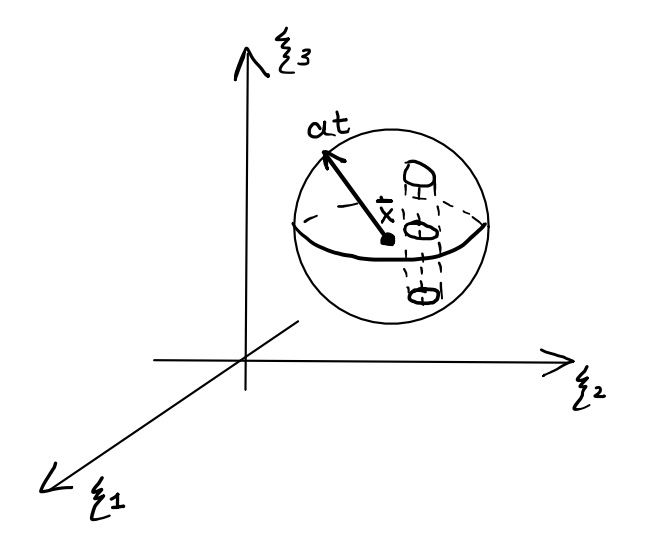
\includegraphics[width=80mm]{cha8im1}
		\columnbreak
		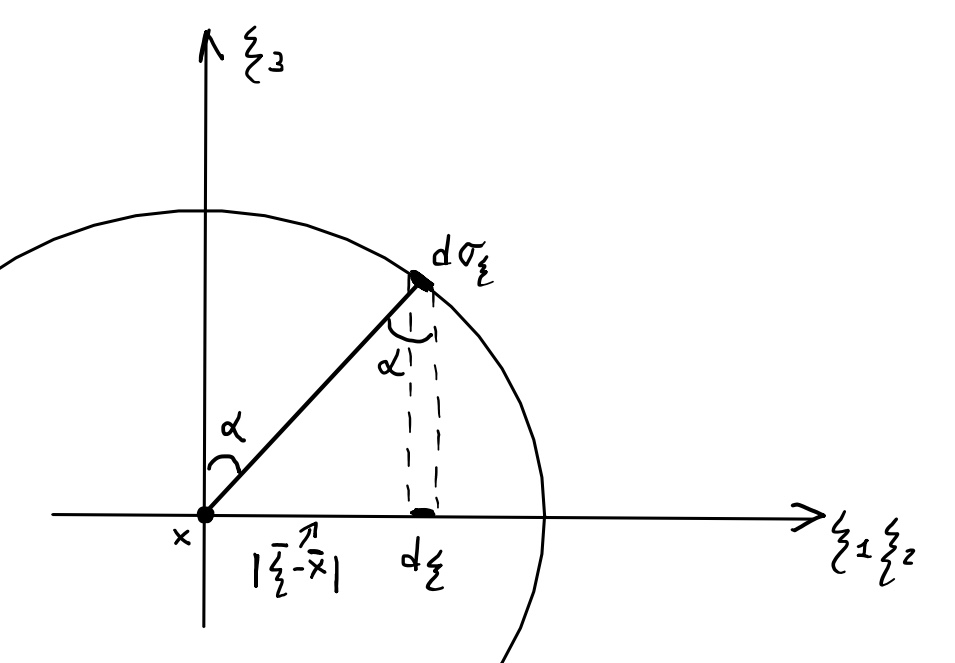
\includegraphics[width=90mm]{cha8im2}
	\end{multicols}
\end{figure}
Сфера проектируется на круг $|\overline{\xi}-\overline{x}|\le at$, $\alpha$ - угол между нормалью к сфере и $\xi_3$, $d \sigma_{\xi}$ - элемент площади на сфере, $d\xi = d\xi_1 d\xi_2$ - элемент площади на круге.
$$\sin{\alpha} = \frac{|\overline{\xi}-\overline{x}|}{a t} \; \Rightarrow \; \cos{\alpha} = \sqrt{1 - \frac{|\overline{\xi}-\overline{x}|^2}{a^2 t^2}} = \frac{\sqrt{a^2t^2|\overline{\xi}-\overline{x}|^2}}{a t} = \frac{d\xi}{d \sigma_{\xi}}$$
Отсюда получаем:
$$u_2 (t, x_1, x_2) = \frac{2}{4\pi a^2 t} \underset{|\overline{\xi}-\overline{x}|\le at}{\overset{}{\iint}}\psi (\xi_1, \xi_2) \frac{d\xi \cdot at}{\sqrt{a^2t^2 - |\overline{\xi}-\overline{x}|^2}} = \frac{1}{2\pi a}\underset{|\overline{\xi}-\overline{x}|\le at}{\overset{}{\iint}} \frac{\psi (\xi_1, \xi_2) d\xi_1 d\xi_2}{\sqrt{a^2t^2 - |\overline{\xi}-\overline{x}|^2}}$$
Умножение на $2$ происходит, потому что в каждую точку круга проецируется две точки сферы (с верхней и нижней частей). Итак, формула Пуассона имеет вид (аналогично формуле Кирхгофа):
$$u(t, \overline{x}) = \frac{1}{2 \pi a} \underset{|\overline{x} - \xi| \leq at}{\overset{}{\iint}} \dfrac{\psi (\overline{\xi}) d \bar{\xi} }{\sqrt{(at)^2 - |\bar{\xi} - \bar{x}|^2}} + \frac{\partial}{\partial t} (\frac{1}{2 \pi a} \underset{|\overline{x} - \xi| \leq at}{\overset{}{\iint}} \dfrac{\varphi (\overline{\xi}) d \bar{\xi} }{\sqrt{(at)^2 - |\bar{\xi} - \bar{x}|^2}}) $$















% Делаем все то же самое, что для формулы Кирхгофа:

% $$\begin{cases}
% 	u_{tt} = a^2 \triangle_{\overline{x}} u, \; t > 0, \; x \in \mathbb{R}^3 \\
% 	u|_{t = 0} = 0 \\
% 	u_t |_{t = 0} = \psi (x_1, x_2)
% \end{cases}$$

% $$
% u(t,x) = \dfrac{1}{2}\underset{|\overline{x} - \xi| \leq at}{\overset{}{\iint}}\dfrac{\psi (\overline{\xi}) d \sigma_\xi }{\sqrt{(at)^2 - |\bar{\xi} - \bar{x}|^2}} 
% $$

% Запишем решение с помощью формулы Кирхгофа для трехмерного случая, считая, что $ \psi = \psi(x_1, x_2): $

% $$
% u(t,x) = \frac{1}{4 \pi a^2 t} \underset{|\overline{x} - \xi| = at}{\overset{}{\varoiint}} \psi (\xi_1, \xi_2) d \sigma_\xi.
% $$

% \begin{center}
% 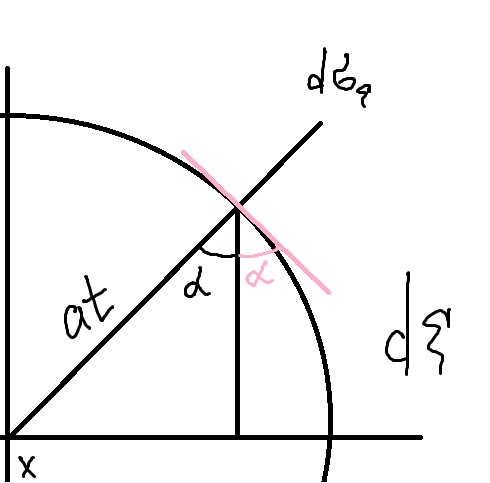
\includegraphics[scale=0.6]{dsigma}
% \end{center}

% $$
% \begin{gathered}
% d\sigma_{\xi} = \dfrac{d\xi}{\cos(\alpha)}, \\
% \sin(\alpha) = \dfrac{|\xi - x|}{at} \longrightarrow \cos(\alpha) = \sqrt{1 - \dfrac{|\xi - x|^2}{(at)^2}} = \dfrac{\sqrt{(at)^2 - |\xi - x|^2}}{at},
% \end{gathered}
% $$

% тогда 

% $$
% u(t, \overline{x}) = \frac{2at}{4 \pi a^2 t} \underset{|\overline{x} - \xi| \leq at}{\overset{}{\iint}} \dfrac{\psi (\overline{\xi}) d \bar{\xi} }{\sqrt{(at)^2 - |\bar{\xi} - \bar{x}|^2}} = \frac{1}{2 \pi a} \underset{|\overline{x} - \xi| \leq at}{\overset{}{\iint}} \dfrac{\psi (\overline{\xi}) d \bar{\xi} }{\sqrt{(at)^2 - |\bar{\xi} - \bar{x}|^2}}
% $$

% В числителе появилась 2, так как в каждую очку круга проецируются две очки сферы (с верхней и нижней частей). Итак, \red{формула Пуассона}:

% $$u(t, \overline{x}) = \frac{1}{2 \pi a} \underset{|\overline{x} - \xi| \leq at}{\overset{}{\iint}} \dfrac{\psi (\overline{\xi}) d \xi_1\xi_2 }{\sqrt{(at)^2 - |\bar{\xi} - \bar{x}|^2}} + \frac{\partial}{\partial t} (\frac{1}{2 \pi a} \underset{|\overline{x} - \xi| \leq at}{\overset{}{\iint}} \dfrac{\varphi (\overline{\xi}) d \bar{\xi} }{\sqrt{(at)^2 - |\bar{\xi} - \bar{x}|^2}}) $$
\end{Proof}

Метод, позволяющий свести задачу большей размерности к задаче меньшей размерности, называется \red{методом спуска}.

\chapter{Устойчивость замкнутой модели Леонтьева.}\label{cha:9}

$$\begin{cases}
	A \pi = \pi \\
	\pi \geq 0
\end{cases} \text{-- замкнутая модель Леонтьева (} \forall \; i: \; \sum\limits_{j = 1}^n a_{ij} = 1 \text{).}$$

Пусть $A \geq 0, \; r_i = \sum\limits_{j = 1}^n a_{ij}, \; s_j = \sum\limits_{i = 1}^n a_{ij}, \; r = \underset{i}{min}r_i, \; R = \underset{i}{max}r_i, \; s = \underset{i}{min}s_i, \; S = \underset{i}{max}s_i$

\begin{clair}
	$A \geq 0 \Rightarrow r \leq \lambda_A \leq R, s \leq \lambda_A \leq S.$
\end{clair}

\begin{conseq}
	$A \geq 0$ -- замкнутая, тогда $\lambda_A = 1.$
\end{conseq}

\begin{definition}
	$A > 0$ -- неразложимая, $\lambda_A = 1$ (иначе $A = \dfrac{1}{\lambda_A}A$). $p_A$ -- левый Фробениусов собственный вектор: $(p_A, p_A) = 1.$
\end{definition}

\begin{definition}
	Норма на $\mathbb{R}^n: \; \| x\|_A = (p_A, |x|), \; |x| = (|x_1|, \ldots, |x_n|).$
\end{definition}

\begin{definition}
	A -- устойчива, если $\forall \; x \; \exists \lim\limits_{k \to \infty}A^k x$
\end{definition}

\begin{remark}
	Выберем правый Фробениусов собственный вектор: $\| x_A\|_A = 1. \; \| Ax\|_A \leq \| x_A\|_A$ и, если $x \geq 0,$ то $\| Ax\|_A = \| x_A\|_A \; (p_A |Ax| \leq p_A A |x| = p_A |x| = \| x \|_A, \; p_A |Ax| = p_A A x = p_A x = p_A |x| = \| x\|_A. )$
\end{remark}

\begin{clair}
	$x \geq 0, $ если $\exists \lim\limits_{k \to \infty}A^k x,$ то $z = \lim\limits_{k \to \infty}A^kx = \mu x_A, \; \mu = \| x\|_A.$
\end{clair}

\begin{definition}[Импримитивная(циклическая) матрица]
	Неразложимая матрица А называется импримитивной(циклической), если $\exists$ разбиение $\{ 1, \ldots, n\} = S_0 \bigsqcup \ldots \bigsqcup S_{m - 1}, \; S_i \cap S_j = \emptyset \; i \neq j, \; \forall i \; S_i \neq \emptyset, $ при этом $a_{ij} > 0 \Rightarrow$:

	$$\begin{cases}
		i \in S_r, \; j \in S_{r - 1}, \; 1 \geq r \geq m - 2 \\
		i \in S_0, \; j \in S_{m - 1}
	\end{cases}$$

	То есть, матрица импримитивна, если одновременной перестановкой столбцов и строк она приводится к виду: 

	\begin{gather*}
		\begin{pmatrix}
		  0 & \ldots & 0 & A_{m-1}\\
		  A_0 & 0 & \ldots & 0\\
		  0 & A_1 & \ldots & 0\\
		  \ldots & \ldots & \ldots & 0\\
		  0 & \ldots & 0 &  A_{m-2}\\
		\end{pmatrix}
	\end{gather*}

	Иначе А -- примитивная.
\end{definition}

\begin{example}
		\begin{gather*}
			\begin{pmatrix}
			  0 & 1\\
			  1 & 0 \\
			\end{pmatrix} \text{--циклическая, неразложимая.}
			\begin{pmatrix}
			  0 & 1\\
			  1 & 1 \\
			\end{pmatrix} \text{--примитивная.}
			\begin{pmatrix}
			  1 & 1\\
			  0 & 1 \\
			\end{pmatrix} \text{--разложимая.}
		\end{gather*}
\end{example}

\begin{theorem}
	Неразложимая матрица $A \geq 0 устойчива, \; \lambda_A = 1 \Longleftrightarrow $ A -- примитивна.
\end{theorem}

\begin{lemma}
	А -- примитивная, тогда у некоторой степени А первая строка положительная: $\exists k: \; \forall \; j a_{1j}^k > 0, \; A^k = (a_{ij}^k)$.
\end{lemma}

\begin{lemma}
	Если матрица $A^k$ устойчива при некотором k, то А -- устойчива.
\end{lemma}

\begin{definition}[Оператор сжатия]
	Оператор Р действует на линейном нормированном пространстве как оператор сжатия, если $\exists \gamma: \; 0 < \gamma < 1: \; \forall \; v \in L: \; \| Pv\| \leq \gamma \| v\|, \; \gamma $ -- коэффициент сжатия. 
\end{definition}

\begin{lemma}
	$L_A:= Ann(p_A) = \{ v | (v, p_A) = 0\}.$ Если оператор А действует на $L_A$ как оператор сжатия, то А -- устойчива.
\end{lemma}

\begin{lemma}
	Если неразложимая матрица А с $\lambda_A = 1$ имеет положительную строку, то оператор А действует на пространстве $L_A:= Ann(p_A) = \{ v | (v, p_A) = 0\}$ как оператор сжатия.
\end{lemma}

\begin{conseq}
	Если неразложимая матрица А с $\lambda_A = 1$ имеет положительную строку, то A -- устойчива.
\end{conseq}

\begin{theorem}
	A > 0 -- неразложимая с $\lambda_A = 1$, тогда А -- устойчивая $ \Longleftrightarrow \forall \; \lambda \in Spec(A) \setminus 1$ выполнено $|\lambda| < 1.$
\end{theorem}
\section{Инвариантная мера. Мера с гладкой плотностью. Плотность при замене координат. Теорема Лиувилля об инвариантной мере. Построение инвариантной меры на многообразии уровней первых интегралов – локально (Существование инвариантной меры у ограничения системы на инвариантное многообразие.)}\label{chasec10}



\newpage
\section{Интегрируемость в квадратурах. Теорема Якоби о последнем множителе.}\label{chasec11}



\newpage
\chapter{Формула Пуассона решения задачи Коши для уравнения теплопроводности.}
\label{cha:12}

$\text{Имеем задачу Коши: }\begin{cases}
	u_{t} = a^2 u_{xx}, \; t > 0, \; x \in \mathbb{R}\\
	u|_{t = 0} = \varphi (x) \\
	|u| \leq C, \; t \geq 0, \; x \in \mathbb{R}.
\end{cases}$

\begin{theorem}[\red{Формула Пуассона}]\label{lec:12/the:1}
	Формула Пуассона решения задачи Коши имеет вид:
	$$u(t, x) = \dfrac{1}{2a\sqrt{\pi t}}\int\limits_{-\infty}^{\infty}e^{-\frac{(x - \xi)^2}{4a^2 t}}\varphi (\xi) d\xi$$
\end{theorem}
\begin{Proof}
Проверим, что формула удовлетворяет уравнению:
$$\left.
  		\begin{array}{ccc}
    		u_t = \dfrac{1}{2a\sqrt{\pi}} \int\limits_{-\infty}^{\infty}(-\dfrac{1}{2t^{\frac{3}{2}}} + \dfrac{1}{\sqrt{t}}\dfrac{(x - \xi)^2}{4a^2t^2})e^{-\frac{(x - \xi)^2}{4a^2t}}\varphi(\xi)d\xi \\
			u_x = \dfrac{1}{2a\sqrt{\pi}} \int\limits_{-\infty}^{\infty} -\dfrac{1}{\sqrt{t}}\dfrac{x - \xi}{2a^2t}e^{-\frac{(x - \xi)^2}{4a^2t}}\varphi(\xi)d\xi \\
			u_{xx} = \dfrac{1}{2a\sqrt{\pi}}\int\limits_{-\infty}^{\infty} (-\dfrac{1}{2a^2t\sqrt{t}} + \dfrac{(x - \xi)^2}{4a^2t^2\sqrt{t}})e^{-\frac{(x - \xi)^2}{4a^2t}}\varphi(\xi)d\xi
  		\end{array}
	\right\} \Rightarrow \;  u_{t} - a^2 u_{xx} = 0$$
Проверим, что удовлетворяет начальным условиям: 
$$\begin{gathered}
	\text{замена: }y = \dfrac{\xi - x}{2a\sqrt{t}} \; \Rightarrow \; \xi = 2a\sqrt{t}y + x, \; d\xi = 2a\sqrt{t}dy \\
	u_t = \dfrac{1}{\sqrt{\pi}} \int\limits_{-\infty}^{\infty} e^{-y^2}\varphi(2a\sqrt{t}y+x)dy \xrightarrow[t\to 0]{} \dfrac{\varphi(x)}{\sqrt{\pi}}\int\limits_{-\infty}^{\infty} e^{-y^2}dy = \varphi(x)
\end{gathered}$$
\end{Proof}

$\text{Имеем многомерную задачу Коши: }\begin{cases}
	u_{t} = a^2 u_{xx}, \; t > 0, \; \bar{x} \in \mathbb{R}^n\\
	u|_{t = 0} = \varphi (\bar{x}) \\
	|u| \leq C, \; t \geq 0, \; \bar{x} \in \mathbb{R}^n.
\end{cases}$

\begin{theorem}[\red{Многомерная формула Пуассона}]\label{lec:12/the:1}
	Формула Пуассона решения многомерной задачи Коши имеет вид:
	$$\begin{gathered}
		u(t, x) = \dfrac{1}{(2a\sqrt{\pi t})^n} \underset{\mathbb{R}^n}{\overset{}{\int_{\dots}\int}} e^{-\frac{|\bar{x} - \bar{\xi}|^2}{4a^2t}}\varphi(\bar{x})d\xi_1\ldots \xi_n,
	\end{gathered}$$
	где $ |\bar{x} - \bar{\xi}|^2 = (x_1 - \xi_1)^2 + \ldots + (x_n - \xi_n)^2. $
\end{theorem}









\chapter{Теорема Вейля. Задание многогранников системой аффинных неравенств}
\label{cha:13}

\epigraph{
	\textit{Пол был землею, потолок — небом, а их соединяли, точно могучие древесные стволы, круглые и многогранные колонны.}}
{-- Куприн А.И.}

\begin{theorem}[\red{Вейля}]\label{cha:13/the:1}
	Конечнопорожденный конус является полиэдром.
\end{theorem}
\begin{Proof}
	Пусть конус $K \subseteq \mathbb{A}^n$ с вершиной O порождается точками $A_1, \dots, A_m$. Можно считать, что $dim K = n$. Пусть O – начало координат и $A_j = (a_{j1}, \dots, a_{jn})$, $1 \le j \le m$. Заметим, что:
	$$n = dim K = dim <\overline{OA_1}, \dots, \overline{OA_m}> = rank 
	\begin{pmatrix}
		a_{11} & \dots & a_{1n} \\
		\vdots & \ddots & \vdots \\
		a_{m1} & \dots & a_{mn}
	\end{pmatrix}\eqno(27)$$
	Предположим, что $B = (b_1, \dots, b_n) \not \in K$. Рассмотрим аффинные функции:
	$$f_j (x_1, \dots, x_n) = \underset{t}{\overset{}{\sum}}a_{jt}x_t, \; j = \ton m \text{ и } g(x_1, \dots, x_n) = \underset{t}{\overset{}{\sum}}b_t x_t$$
	По теореме Фаркаша неравенство $g \ge 0$ не является следствием совместной системы неравенств (5). Следовательно, найдется такая точка $z = (z_1, \dots, z_n) \in \mathbb{A}^n$, что:
	$$f_1 (z) \ge 0, \dots, f_m (z) \ge 0, \; g(z) = a < 0$$
	Рассмотрим полиэдр $P^0$, задаваемый системой неравенств:
	$$f_1 \ge 0, \dots, f_m \ge 0, \; -g + a \ge 0\eqno(28)$$
	Полиэдр $P^0$ непуст, так как он содержит точку z. По теореме Фань Цзы и (27) полиэдр $P^0$ имеет вершину $C = (c_1, \dots, c_n)$. Среди неравенств (28) n линейно независимых функций должны обращаться в нуль. Если n линейно независимых функций среди $f_1, \dots, f_m$ обращается в точке C в нуль, то в силу определения функций $f_1, \dots, f_m$, получаем, что точка C – начало координат. В этом случае $−g(C) + a = a < 0$, что невозможно. Итак, только $n − 1$ независимая функция среди $f_1, \dots, f_m$, обращается в нуль. Кроме того, $−g(C) + a = 0$.

	Рассмотрим уравнение $h(x) = c_1x_1 + \dots + c_nx_n = 0$. По построению $n − 1$ точка среди $A_1, \dots, A_m$ удовлетворяет этому уравнению. Для остальных точек $A_j$ получаем $h(A_j) > 0$. Кроме того, $h(B) = g(C) = a < 0$. Итак, плоскость $\Pi$, задаваемая уравнением $h(x) = 0$ разделяет K и B, причем $\Pi \cap K$ является гранью размерности $n − 1$. Тем самым эти грани определяют полупространства, пересечением которых совпадает с K. Эти полупространства связаны с выбором $n−1$ независимой точки среди $A_1, \dots, A_m$ и проходят через эти точки и начало координат.
\end{Proof}

\begin{theorem}[]\label{cha:13/the:2}
	Конечнопорожденный многогранник является полиэдром.
\end{theorem}
\begin{Proof}
	Пусть многогранник M порождается точками:
	$$A_1, \dots, A_m\eqno(29)$$
	и $\Pi$ – наименьшая плоскость, содержащая M. Можно считать, что $\Pi = \mathbb{A}^n$. Вложим $\mathbb{A}^n$ в $\mathbb{A}^{n+1}$ и возьмем точку $O \in \mathbb{A}^{n+1} \ \mathbb{A}^n$. Пусть K – конус с вершиной O, порожденный точками (29). Заметим, что множество $K \cap \Pi$ выпукло и содержит точки (29). Следовательно, $M \subseteq K \cap \Pi$. Покажем, что $K \cap \Pi \subseteq M$. Выберем в $\mathbb{A}^{n+1}$ систему координат с началом в O и с базисом $e_0, \dots, e_n$, причем $e_0 = \overline{OA_1}$ и $<e_1, \dots, e_n> = <\overline{A_1 A_2}, \dots, \overline{A_1 A_m}>$. Тогда $\Pi = A_1 + <e_1, \dots, e_n>$. Рассмотрим точку:
	$$A = O + \lambda_1 \overline{OA_1} + \dots + \lambda_m \overline{OA_m} \in K \cap \Pi, \; \lambda_1, \dots, \lambda_m \ge 0$$
	Тогда:
	$$\begin{gathered}
		A = O + \lambda_1 \overline{OA_1} + \dots + \lambda_m \overline{OA_m} = O + \left( \underset{i=1}{\overset{m}{\sum}}\lambda_i \right) \overline{OA_1} + \underset{i \ge 2}{\overset{}{\sum}}\lambda_i \overline{A_1 A_i} \in \Pi = \\
		= A_1 + <e_1, \dots, e_n> = O + \overline{OA_1} + <e_1, \dots, e_n>
	\end{gathered}$$
	Отсюда $\underset{i=1}{\overset{m}{\sum}}\lambda_i = 1$ и $A \in M$ по предложению \ref{cha:11/propose:1}. Итак, $M = K \cap \Pi$. Поэтому M задается неравенствами, определяющими K и уравнениями, определяющими $\Pi$.
	
\end{Proof}

















\chapter{Обобщенные функции. Действия над обобщенными функциями. Фундаментальное решение линейного дифференциального оператора с постоянными коэффициентами.}
\label{cha:14}

\begin{definition}
	\red{Финитная функция $ \varphi(x) $: }
	$\varphi(x) =
	\begin{cases}
		\neq 0, \; x \in K\\
		\equiv 0, \; x \notin K
	\end{cases}$
	
	где $K \subset \Omega $ - компакт и носитель функции $ \varphi(x) .$
\end{definition}

\begin{definition}
	\red{Основные(пробные) функции} -- бесконечно дифференцируемые финитные функции.
\end{definition}

\begin{definition}
	$ D(\Omega) = C_0^{\infty}(\Omega) $ -- \blue{множество бесконечно дифференцируемых функций}.
\end{definition}

\begin{definition}
	$ \varphi_n(x) \in D(\Omega) \underset{\text{равномерно}}{\longrightarrow} \varphi(x), $ если:
	\begin{enumerate}
		\item $ 
			\exists \; K: \; K_n \subseteq K \subset \Omega, \; K_n $ -- носитель $ \varphi_n(x)$
		\item 
			$ \dfrac{\partial^{|\alpha|}\varphi_n(x)}{\partial x^{\alpha}} \underset{K}{\rightrightarrows} \dfrac{\partial^{|\alpha|}\varphi(x)}{\partial x^{\alpha}}, \; |\alpha| = 0,\; 1, \ldots, \text{т.е. } \dfrac{\partial^{|\alpha|}}{\partial x^{\alpha}} \equiv \dfrac{\partial^{\alpha_1 + \ldots + \alpha_n}}{\partial x_1^{\alpha_1}\ldots\partial x_n^{\alpha_n}}.$
	\end{enumerate}
\end{definition}

\begin{definition}
	\red{Обобщенные функции} -- линейные непрерывные функционалы над $ D(\Omega). $ \textit{Обозначение: } $ D'(\Omega) $ или $ D^{*}(\Omega) .$
\end{definition}

\begin{definition}
	\red{Функционал: } L: $ \varphi(x) \in D(\Omega) \to \mathbb{R}. $
\end{definition}

\begin{definition}
	\blue{Линейный функционал: } $ L(\varphi_1(x)\alpha + \varphi_2(x)\beta) = \alpha L(\varphi_1(x)) + \beta L(\varphi_2(x)).$
\end{definition}

\begin{definition}
	\blue{Непрерывный функционал: } $ \varphi_n(x) \underset{\text{равномерно}}{\longrightarrow} \varphi(x) \Longrightarrow L(\varphi_n(x)) \longrightarrow L(\varphi(x))$
\end{definition}

\begin{definition}
	\red{$L_{1loc}$ } -- интегрируемые на $ \forall $ компакте $K \subset \Omega. $
\end{definition}

\begin{theorem}
	$ \forall L \; \exists f(x) \in L_{1loc}: \; \forall \; \varphi(x) \in D \; L(\varphi(x)) = (f(x), \varphi(x)), $ где
	$$\begin{gathered}
		(f(x), \varphi(x)) = \int\limits_{\Omega} f(x)\varphi(x)dx.
	\end{gathered}$$
\end{theorem}

\begin{definition}
	\blue{Регулярные обобщенные функции}: 
	$$\text{функционалы } L: \; \exists f(x) \in  L_{1loc}(\Omega): \; \forall \; \varphi(x)\in D(\Omega)$$
	$$\begin{gathered}
		(f(x), \varphi(x)) = \int\limits_{\Omega} f(x)\varphi(x)dx.
	\end{gathered}$$
\end{definition}

\begin{definition}
	\blue{Сингулярные обобщенные функции }: 
	$$\begin{gathered}
		\text{функционалы } L: \; \nexists f(x) \in  L_{1loc}(\Omega): \; L(\varphi(x)) = (f(x), \varphi(x))
	\end{gathered}$$
\end{definition}

\begin{definition}
	\red{Дельта-функция}: 
	$\delta(x) =
	\begin{cases}
		0, \; x \neq 0\\
		\infty, \; x = 0
	\end{cases}$
	$$\delta(\varphi) = \varphi(0) = (\delta, \varphi) = (\delta(x), \varphi(x)) =  \int\limits_{\Omega} \delta(x)\varphi(x)dx$$
\end{definition}

\section*{Действия с обобщенными функциями}

\begin{enumerate}
	\item \underline{Линейная комбинация} обобщенных функций:
		$$\begin{gathered}
			f_1(x), \; f_2(x) \in D'(\Omega) \; \Rightarrow \;  \forall \; \alpha, \; \beta \in \mathbb{R} \; \alpha f_1(x) + \beta f_2(x) \in D'(\Omega) \\
			(\alpha f_1(x) + \beta f_2(x), \varphi(x)) = \alpha (f_1, \varphi) + \beta (f_2, \varphi) \; \forall \varphi \in D.
		\end{gathered}$$
	\item \underline{Линейная замена переменных} в аргументе обобщенных функций:
		$$\begin{gathered}
			f \in D'(\Omega) \; \Rightarrow \;  f(Ax + b) \in D'(\Omega), \; det(A) \neq 0 \\
			(f(Ax + b), \varphi(x)) \equiv \dfrac{1}{|A|} (f(x), \varphi(A^{-1}(x - b)))
		\end{gathered}$$
		Рассмотрим $\mathbb{R}^1$: пусть $f(x)$ - регулярная функция, тогда:
		$$\begin{gathered}
			(f(Ax + b), \varphi(x)) = \int\limits_{R}f\underbrace{(Ax + b)}_{= y}\varphi(x)dx = \dfrac{1}{|A|}\int\limits_{R}f(y)\varphi(\frac{y - b}{A})dy
		\end{gathered}$$
		Для $\mathbb{R}^n$ аналогично: $A^{-1}$ - обратная матрица, $\frac{1}{|A|}$ - якобиан многомерной линейной замены переменных.
	\item \underline{Умножение обобщенной функции} на бесконечно дифференцируемую функцию:
		$$\begin{gathered}
			f(x) \in D'(\Omega), \; a(x) \in C^{\infty}(\Omega) \longrightarrow a(x)f(x) \in D'(\Omega) \\
			(a(x)f(x), \varphi(x)) = (f(x), a(x)\varphi(x))
		\end{gathered}$$
		Если $f(x)$ - регулярная, то $(a(x)f(x), \varphi(x)) = \int\limits_{\Omega} a(x)f(x) \varphi(x) dx$.
	\item \underline{Дифференцирование} обобщенной функции: $ f(x) \in D'(\Omega). $
		Рассмотрим $\mathbb{R}^1$: 
		$$\begin{gathered}
			f'(x) \in D(\Omega): \; (f'(x), \varphi(x)) \equiv - (f(x), \varphi'(x)) \\
			(f^{(k)}(x), \varphi(x)) \equiv (-1)^k(f(x), \varphi^{(k)}(x))
		\end{gathered}$$

		Если $f(x)$ - регулярная, то:
		$$\begin{gathered}
			(f', \varphi) = \int\limits_{-\infty}^{\infty}
			f'(x)\varphi(x)dx = \int\limits_{-\infty}^{\infty} \varphi(x)df(x) = \underbrace{f(x)\varphi(x) \mid_{-\infty}^{\infty}}_{ 0 \text{, т.к. } \varphi \text{ -- финитная}} - \int\limits_{-\infty}^{\infty} f(x)\varphi'(x)dx
		\end{gathered}$$
\end{enumerate}

\section*{Свертка обобщенных функций}

Пусть $f(x), \; g(x) \in L_1$. Тогда верны следующие свойства:

\begin{enumerate}
	\item 
		$ (f * g)(x) = \int\limits_{-\infty}^{\infty} f(t)g(x - t)dt = (g * f)(x)$ 
	\item 
		$ (f * g)'(x) = (f' * g)(x) = (f * g')(x)  $
	\item 
		$ (f * g)^{m}(x) = (f^{k} * g^{m - k})(x) = (f^{m - k} * g^{k})(x)  $
	\item 
		$ f(x), \; g(x) \in D' \; \Rightarrow \;  (f * g)(x) \in D': $
		\begin{Proof}
			$$\begin{gathered}
			((f * g)(x), \varphi(x)) \equiv (f(x), (g(x), \varphi(x + t))_t) \; \\ 
			\forall \varphi(x) \in D \\
			((f * g)(x), \varphi(x)) = \int\limits_{-\infty}^{\infty} \varphi(x) (\int\limits_{-\infty}^{\infty} f(t)g(t - x)dt)dx =\\
			= \int\limits_{-\infty}^{\infty} f(t) (\int\limits_{-\infty}^{\infty} g(t - x)\varphi(x))dtdx = \int\limits_{-\infty}^{\infty} f(t) (\int\limits_{-\infty}^{\infty} g(y)\varphi(y + t))dtdy
			\end{gathered}$$
		\end{Proof}
	\item 
		$ ((f * g)'(x), \varphi(x)) =  -((f * g)(x), \varphi'(x))$
		\begin{Proof}
			$$ ((f * g)'(x), \varphi(x)) =  -((f * g)(x), \varphi'(x)) = (f(x), (g(x), \varphi'(x + t))_t)_x = $$
			\begin{itemize}
				\item[$\bullet$] 
					$= (f(x), (g'(x), \varphi(x + t))_t)_x = ((f * g')(x), \varphi(x)) $
				\item[$\bullet$] 
					$= -(f(x), (g(x), \dfrac{\partial}{\partial x}\varphi(x + t))_t)_x = -(f(x), \dfrac{\partial}{\partial x}(g(x), \varphi(x + t))_t)_x = \\
					= (\dfrac{\partial}{\partial x}f(x), (g(x), \varphi(x + t))_t)_x = ((f' * g)(x), \varphi(x))$
			\end{itemize}
		\end{Proof}
\end{enumerate}

\section*{Фундаментальное решение дифференциального оператора}

Имеем дифференциальное уравнение и дифференциальный оператор:
$$\begin{gathered}
	Ly \equiv y^{(m)} + a_{m - 1}y^{(m - 1)} + \dots a_1y' + a_0y = f(x) \\
	L \equiv \dfrac{d^m}{dx^m} + a_{m - 1}\dfrac{d^{m - 1}}{dx^{m - 1}} + \dots + a_1\dfrac{d}{dx} + a_0
\end{gathered}$$

\begin{definition}
	$ \varepsilon(x) \in D' $ -- \red{фундаментальное решение дифференциального оператора L}, если $ L\varepsilon(x) = \delta(x) $.
\end{definition}

\begin{remark}
	Если $y_0$ - решение, т.е. $Ly_0 = 0$, тогда $\varepsilon(x) + y_0$ - фундаментальное решение.
\end{remark}

\begin{definition}
	$ \theta(x) $ -- \red{функция Хевисайда:}
	$$\theta(x) = 
	\begin{cases}
		1, \; x \geq 0\\
		0, \; x < 0
	\end{cases} \text{и } \theta'(x) = \delta(x)$$
\end{definition}

\begin{theorem}[\blue{нахождение фундаментального решения}]\label{lec:13/the:2}
	Формула нахождения фундаментального решения имеет вид: $ \varepsilon(x) = \theta(x)u(x), $ где $ u(x) $ является решением системы: 
	$$\begin{gathered}
		\begin{cases}
			Lu(x) = 0\\
			u(0) = 0\\
			u'(0) = 0 \\
			\ldots\\
			u^{(m-2)}(0) = 0\\
			u^{(m-1)}(0) = 1\\
		\end{cases}
	\end{gathered}$$
\end{theorem}
\begin{Proof}
	\begin{flushleft}
		$\varepsilon'(x) = \theta'(x)u(x) + \theta(x)u'(x) = \delta(x)u(x) + \theta(x)u'(x) =$
		
		\hspace{1.15cm}$= \delta(x)u(0) + \theta(x)u'(x) = \theta(x)u'(x)$

		$\varepsilon''(x) = \theta'(x)u'(x) + \theta(x)u''(x) = \theta(x)u''(x)$

		$\dots$
		
		$\varepsilon^{(m - 1)}(x) = \theta(x)u^{(m - 1)}(x)$

		$\varepsilon^{(m)}(x) = \theta'(x)u^{(m - 1)}(x) + \theta(x)u^{(m)}(x) = \delta(x)u^{(m - 1)}(x) + \theta(x)u^{(m)}(x) =$

		\hspace{1.5cm} $= \delta(x)u^{(m - 1)}(0) + \theta(x)u^{(m)}(x) = \delta(x) + \theta(x)u^{(m)}(x)$
	\end{flushleft}
	Тогда получаем:
	$$\begin{gathered}
		L\varepsilon(x) = \delta(x) + \theta(x)u^{(m)}(x) + a_{m - 1}\theta(x)u^{(m - 1)}(x) + \ldots + a_1\theta(x)u'(x) + a_0\theta(x)u(x) = \\
		= \theta(x)(L(u(x))) + \delta(x) = \delta(x).
	\end{gathered}$$
\end{Proof}












\chapter{Теорема о системах линейных неравенств.}\label{cha:15}

\begin{theorem}
	Пусть $X = \{ x \geq 0 | Ax \leq b\} \neq \emptyset$ и $\forall \; x \in X: \; (c, x) \leq d \Rightarrow \exists p \geq 0: \; pA \geq c, \; (p, b) \leq d.$
\end{theorem}


\chapter{Фундаментальное решение оператора Лапласа в $R^2$ и $R^3$.}
\label{cha:16}

Рассмотрим оператор Лапласса: $L = \triangle = \frac{\partial^2}{\partial x_1^2} + \dots + \frac{\partial^2}{\partial x_n^2}$.

\begin{theorem}[\red{Фундаментальное решение оператора Лапласса}]\label{lec:16/the:1}
	Фундаментальное решение оператора Лапласса имеет вид:
	$$ \varepsilon (x) = 
	\begin{cases}
		\displaystyle \frac{1}{2 \pi} \ln |\vec{x}|, \; \vec{x} \in \mathbb{R}^2\\
		\displaystyle - \frac{1}{4 \pi |\vec{x}|}, \; \vec{x} \in \mathbb{R}^3 \\
		\displaystyle -\frac{1}{\sigma_n |\vec{x}|^{n-2}}, \; \vec{x} \in \mathbb{R}^n , n \ge 4 
	\end{cases}$$
	где $\sigma_n$ - площадь поверхности единичной сферы в $\mathbb{R}^n$.
\end{theorem}
\begin{Proof}
	Необходимо проверить, что $\triangle \varepsilon (x) = \delta (x) $, т.е. что:
	$$(\triangle \varepsilon (x) , \varphi (x)) = (\delta (x), \varphi (x)) = \varphi (0)$$
	1) Рассмотрим \blue{$\mathbb{R}^2$}, то есть когда $\varepsilon (x) = \displaystyle \frac{1}{2 \pi} \ln |\vec{x}|$.
	$$\begin{gathered}
		(\triangle \varepsilon (x) , \varphi (x)) = (\varepsilon_{x_1 x_1} + \varepsilon_{x_2 x_2} , \varphi (x)) = (\varepsilon (x), \varphi_{x_1 x_1} + \varphi_{x_2 x_2}) = \\
		= (\varepsilon (x) , \triangle \varphi (x)) = \iint \limits_{\mathbb{R}^2} \varepsilon (x) \triangle \varphi (x) d \vec{x} = \lim_{\alpha \to 0} \iint \limits_{\alpha < |\vec{x}| < R} \varepsilon (x) \triangle \varphi (x) d \vec{x} =  \\
		=\Big|\text{2-ая формула Грина}\Big|
		= \lim_{\alpha \to 0} \left(\iint \limits_{\alpha < |\vec{x}| < R} \varphi (x) \triangle \varepsilon (x) d \vec{x} + \oint \limits_{|\vec{x}| = \alpha} (\varepsilon \frac{\partial \varphi}{\partial \vec{n}} - \varphi \frac{\partial \varepsilon}{\partial \vec{n}}) d \sigma\right)
	\end{gathered}$$
	(интеграл $\oint \limits_{|\vec{x}| = R}=0$ , т.к. в силу финитности $\varphi \equiv 0$ на $|x| = R$)

	Введем обозначения:
	$$I_1 =  \iint \limits_{\alpha < |\vec{x}| < R} \varphi (x) \triangle \varepsilon (x) d \vec{x}, \; I_2 = \oint \limits_{|\vec{x}| = \alpha} \varepsilon \frac{\partial \varphi}{\partial \vec{n}} d \sigma, \; I_3 = - \oint \limits_{|\vec{x}| = \alpha} \varphi \frac{\partial \varepsilon}{\partial \vec{n}} d \sigma$$
	Рассмотрим $I_1$. Перейдем в полярные координаты, тогда оператор Лапласса записывается следующим образом:
	$$ \triangle = \frac{\partial^2}{\partial \rho^2} + \frac{1}{\rho} \frac{\partial}{\partial \rho} \left(+ \frac{1}{\rho^2} \frac {\partial^2}{\partial \theta^2}\right) $$
	Так как $\varepsilon = \varepsilon (\rho)$, т.е. не зависит от $\theta$, то $\left(+ \frac{1}{\rho^2} \frac {\partial^2}{\partial \theta^2}\right)$ не нужно.
	$$\triangle \varepsilon = (\frac{\partial^2}{\partial \rho^2} + \frac{1}{\rho} \frac{\partial}{\partial \rho}) (\frac{1}{2 \pi} \ln \rho) = \frac{1}{2 \pi} (\frac {1}{\rho} \frac {1}{\rho} - \frac {1}{\rho^2}) = 0$$
	Таким образом, $I_1 = 0$, т.к. в кольце $(\alpha < \rho < R)$ нет нуля.\\

	Рассмотрим $I_2$:
	$$\begin{gathered}
		I_2 = \int \limits_0^{2 \pi} (\varepsilon \frac{\partial \varphi}{\partial \vec{n}} \rho) |_{\rho = \alpha} d \theta = \Big| \rho \text{ - якобиан полярной замены}\Big| = \\
		= \frac{1}{2 \pi} \int \limits_0^{2 \pi} (\ln \rho \frac{\partial \varphi}{\partial \vec{n}} \rho) |_{\rho = \alpha} d \theta  = \frac{1}{2 \pi} \alpha \ln \alpha \underbrace{\int \limits_0^{2 \pi} \frac{\partial \varphi}{\partial \vec{n}}d \theta}_{= const} \xrightarrow[\alpha \to 0]{} 0
	\end{gathered}$$
	Рассмотрим $I_3$. На внутренней границе $\displaystyle \frac{\partial}{\partial \vec{n}} = -\frac{\partial}{\partial \rho}$. Тогда:
	$$\begin{gathered}
		I_3 = - \int \limits_0^{2 \pi} (\varphi (- \frac{\partial \varepsilon}{\partial \vec{n}}) \rho) |_{\rho = \alpha} d \theta =  \int \limits_0^{2 \pi} (\varphi \frac{1}{2 \pi \rho} \rho) |_{\rho = \alpha} d \theta  = \frac{1}{2 \pi} \int \limits_0^{2 \pi} \varphi (\rho, \theta) |_{\rho = \alpha} d \theta = \\
		= \frac{1}{2 \pi} \int \limits_0^{2 \pi} \varphi (\alpha, \theta) d \theta = \underbrace{\frac{1}{2 \pi} \varphi (\alpha, \theta^{*}) \int \limits_0^{2 \pi} d \theta}_{\text{теорема о среднем}} = \varphi (\alpha, \theta^{*}) \xrightarrow[\alpha \to 0]{} \varphi (0)
	\end{gathered}$$\newpage
	2) Рассмотрим \blue{$\mathbb{R}^3$}, то есть когда $\varepsilon (x) = \displaystyle - \frac{1}{4 \pi |\vec{x}|}, \; \vec{x} \in \mathbb{R}^3$.
	$$\begin{gathered}
		(\triangle \varepsilon (x) , \varphi (x)) = (\varepsilon_{x_1 x_1} + \varepsilon_{x_2 x_2} + \varepsilon_{x_3 x_3}, \varphi (x)) = (\varepsilon (x), \varphi_{x_1 x_1} + \varphi_{x_2 x_2} + \\
		\varphi_{x_3 x_3}) = (\varepsilon (x) , \triangle \varphi (x)) = \iiint \limits_{\mathbb{R}^3} \varepsilon (x) \triangle \varphi (x) d \vec{x} = \lim_{\alpha \to 0} \iiint \limits_{\alpha < |\vec{x}| < R} \varepsilon (x) \triangle 		\varphi (x) d \vec{x} =  \\
		=\Big|\text{2-ая формула Грина}\Big|
		= \lim_{\alpha \to 0} \left(\iiint \limits_{\alpha < |\vec{x}| < R} \varphi (x) \triangle \varepsilon (x) d \vec{x} + \oint \limits_{|\vec{x}| = \alpha} (\varepsilon \frac{\partial \varphi}{\partial \vec{n}} - \varphi \frac{\partial \varepsilon}{\partial \vec{n}}) d \sigma\right) = \\
		= \lim_{\alpha \to 0} \left(\underbrace{\iiint \limits_{\alpha < |\vec{x}| < R} \varphi (x) \triangle \varepsilon (x) d \vec{x}}_{I_1} + \underbrace{\oint \limits_{|\vec{x}| = \alpha} \varepsilon \frac{\partial \varphi}{\partial \vec{n}} d \sigma}_{I_2} + \underbrace{\oint \limits_{|\vec{x}| = \alpha}  -\varphi \frac{\partial \varepsilon}{\partial \vec{n}} d \sigma}_{I_3} \right)
	\end{gathered}$$
	\begin{itemize}
		\item $I_1 = \iiint \limits_{\alpha < |\vec{x}| < R} \varphi (x) \triangle \varepsilon (x) d \vec{x} = 0$, так как 
		$$\begin{gathered}
			\varepsilon = -\dfrac{1}{4\pi \rho}, \; \triangle\varepsilon = \varepsilon_{\rho\rho} + \dfrac{2}{\rho}\varepsilon_{\rho} \\
			\varepsilon_{\rho} = \dfrac{1}{4\pi\rho^2}, \; \varepsilon_{\rho\rho} = \dfrac{-2}{4\pi\rho^3} \Longrightarrow \triangle\varepsilon = 0
		\end{gathered}$$
		\item $I_2 = \oint \limits_{|\vec{x}| = \alpha} \varepsilon \dfrac{\partial \varphi}{\partial \vec{n}}d\sigma $. Сделаем замену:
		$$\begin{gathered}
			\begin{cases}		
				x_1 = \rho \sin\theta\cos\phi \\	
				x_2 = \rho \sin\theta\sin\phi \\	
				x_3 = \rho \cos\theta
			\end{cases},  \theta \in [0, \pi], \; \phi \in [0, 2\pi), 
			\mathbb{J} = 
			\begin{vmatrix}
				x_{1\rho} & x_{1\theta} & x_{1\phi}  \\
				x_{2\rho} & x_{2\theta} & x_{2\phi}  \\
				x_{3\rho} & x_{3\theta} & x_{3\phi}  \\
			\end{vmatrix} =
			\rho^2\sin\theta,
		\end{gathered}$$
		тогда
		$$\begin{gathered}
			I_2 = -\int\limits_{0}^{2\pi} \int\limits_{0}^{\pi} \varepsilon \dfrac{\partial \varphi}{\partial \rho}|_{\rho = \alpha}(\rho^2\sin\theta)
			|_{\rho = \alpha} d\theta d\phi = \\
			= \dfrac{\alpha^2}{4\pi\alpha} \int\limits_{0}^{2\pi} \int\limits_{0}^{\pi}  \dfrac{\partial \varphi}{\partial \rho}|_{\rho = \alpha}\sin\theta
			d\theta d\phi = \dfrac{\alpha}{4\pi} const \underset{\alpha \rightarrow 0}{\longrightarrow} 0
		\end{gathered}$$
		\item $ I_3 = - \oint \limits_{|\vec{x}| = \alpha} \varphi \dfrac{\partial \varepsilon}{\partial \rho} d \sigma $ 
		$$\begin{gathered}
			 I_3 = \dfrac{\alpha^2}{4\pi\alpha^2} \int\limits_{0}^{2\pi} \int\limits_{0}^{\pi} \varphi(\alpha, \theta, \phi) \sin\theta d\theta d \phi = \\
			 = \Big|\text{теорема о среднем}\Big| = 
			 \dfrac{1}{4\pi} \int\limits_{0}^{2\pi} \varphi(\alpha, \theta^{*}, \phi)\underbrace{\int\limits_{0}^{\pi} \sin\theta d\theta }_{= -\cos\theta|_{0}^\pi 
			 = 2} d\phi = \\
			 = \dfrac{1}{2\pi} \int\limits_{0}^{2\pi} \varphi(\alpha, \theta^{*}, \phi) d\phi = \varphi(\alpha, \theta^{*}, \phi^{*}) \underset{\alpha \rightarrow 
			 0}{\longrightarrow} \varphi(0,0,0), \; \theta^{*} \in [0, \pi], \; \phi^{*} \in [0, 2\pi)
		\end{gathered}$$
	\end{itemize}
\end{Proof}








\chapter{Теорема Моришимы о магистралях.}\label{cha:17}

A, B -- неотрицательные матрицы $m \times m$. Рассмотрим последовательность интенсивностей: $x_1, \ldots, x_r, \ldots, \; x_t \in \mathbb{R}^m_+, Ax_t \text{-- вектор затрат, } Bx_t \text{-- вектор выпуска.}$

\begin{definition}[Условие замкнутости]
	$Ax_t \leq Bx_{t-1} \Rightarrow x_1, \ldots, x_t$ -- траектория.
\end{definition}

\begin{problem}
	$$\begin{cases}
		<c, x_T> \to \max\\
		Ax_t \leq B x_{t - 1}, \; t = 2, \ldots, T\\
		x_t \geq 0
	\end{cases}$$ Решение этой задачи -- оптимальная траектория.
\end{problem}

\begin{remark}
	Если $c = qB, \; q \geq 0 \text{ -- вектор цен, } <c, x_T> = qBx_{T}$ -- стоимость выпуска $Bx_T.$
\end{remark}

\begin{sign}
	$x, y \in \mathbb{R}^m, \; y \neq 0, \; s(x, y) = \| \dfrac{x}{\| x \|} - \dfrac{y}{\| y \|}\|$ -- расстояние между направлениями x и y.
\end{sign}

\begin{definition}[Магистраль]
	В задаче выше -- это вектор $x \neq 0: \; \forall \; \varepsilon > 0 \exists T_1(\varepsilon), T_2(\varepsilon): \; \forall \; t: \; T_1(\varepsilon) \leq t \leq T - T_2(\varepsilon) \; \forall \text{ оптимальной траектории } \{ x_t\}: \; s(x_t, \vec{x}) < \varepsilon.$
\end{definition}

\begin{definition}[Слабая магистраль]
	Это вектор $x: \; \forall \; \varepsilon > 0 \exists Q(\varepsilon) \in \mathbb{N}: \forall \text{ оптимальной траектории } \{ x_t\} \text{ неравенство } s(x_t, \vec{x}) < \varepsilon \text{ нарушается } \leq Q(\varepsilon) \text{ раз.}$
\end{definition}

\begin{problem}
	Дано: m = n, B = I -- единичная матрица, А -- неразложимая, примитивная, $c \gg 0, \; x_0 \gg 0$. 

	$$\begin{cases}
		<c, x_T> \to \max\\
		Ax_t \leq B x_{t - 1}\\
		x_t \geq 0
	\end{cases}$$ 
\end{problem}

\begin{lemma}
	A -- неразложимая, примитивная $\Rightarrow \exists T_1: \; \forall \; t \geq T_1: \; A^t \gg 0.$
\end{lemma}

\begin{lemma}
	$s(x, y) < 2\dfrac{\| x - y\|}{\| x\|}.$
\end{lemma}

\begin{lemma}
	A -- неразложимая, примитивная $\Rightarrow \forall \; \varepsilon > 0: \; \exists T_2(\varepsilon): \; \forall \; t \geq T_2 \; \forall \; x > 0 \; s(A^t, x_A) < \varepsilon.$
\end{lemma}

\begin{theorem}[Теорема Моришимы]
	В задаче номер 3 $x_A$ -- магистраль.
\end{theorem}

\begin{remark}
	$T_1$ зависит только от А, $T_2$ зависит от А и $\varepsilon$, но оба не зависят от $x_0, c, T, \{ x_t\}_{t = 1}^T.$
\end{remark}
\section{Свойства уравнений Гамильтона интеграл энергии; циклические интегралы и понижение порядка в уравнениях Гамильтона; инвариантная мера уравнений Гамильтона (теорема Лиувилля о сохранении фазового объема)}\label{chasec18}



\newpage

\cleardoublepage
\phantomsection
\addcontentsline{toc}{chapter}{Список используемой литературы}
\begin{thebibliography}{}
	\bibitem{0}
		Курс лекций И.М.Никонова, механико-математический факультет МГУ им. М.В.Ломоносова, 2021 г.
	\bibitem{1}
		Курс семинаров И.М.Никонова, механико-математический факультет МГУ им. М.В.Ломоносова, 2021 г.
\end{thebibliography}

\end{document}
